\documentclass[preprint,12pt]{elsarticle}

\usepackage[utf8]{inputenc}
\usepackage[english]{babel}
\usepackage{graphicx}
\usepackage{subcaption}
\usepackage{booktabs}
\usepackage{amsmath}
\usepackage{amsfonts}
\usepackage{amssymb}
\usepackage{hyperref}
\usepackage{xurl}
\usepackage{ragged2e}
\usepackage{array}
\usepackage{xcolor}
\usepackage{geometry}
\usepackage{longtable}
\usepackage{microtype}
\usepackage{tikz}
\usetikzlibrary{shapes.geometric, arrows.meta, positioning, fit, backgrounds, calc}
\usepackage{float}
\usepackage[colorinlistoftodos]{todonotes}

\geometry{a4paper, margin=2.5cm}

\newcolumntype{P}[1]{>{\RaggedRight\arraybackslash}p{#1}}

\journal{Journal of Informetrics}

\newcommand{\joao}[1]{\todo[color=blue!20, inline]{João: #1}}

\begin{document}

\begin{frontmatter}

  \title{OpenSciencePipe: An End-to-End Framework for Autonomous Science Mapping and Systematic Evidence Synthesis}
\author[inst1]{João Garcia Farinha\corref{cor1}}
\ead{jgfarinha@ciencias.ulisboa.pt}
\cortext[cor1]{Corresponding author}
\author[inst1]{Carlos Duarte}
\ead{cduarte@ciencias.ulisboa.pt}

\affiliation[inst1]{organization={LASIGE, Faculdade de Ciências, Universidade de Lisboa},
            addressline={Campo Grande}, 
            city={Lisboa},
            postcode={1749-016},
            country={Portugal}}

\begin{abstract}
Quantitative research synthesis is historically bifurcated between exploratory science mapping (e.g., VOSviewer, CiteSpace) and confirmatory evidence synthesis (e.g., Cochrane RevMan, \texttt{metafor}). Both workflows encounter fragmented toolchains, manual export bottlenecks, CPU scalability limits on large citation graphs, and heuristic models that discard semantic context. We introduce \textbf{OpenSciencePipe}, an open-source computational framework uniting exploratory bibliometric discovery and confirmatory meta-analysis into an autonomous, reproducible pipeline. OpenSciencePipe integrates multi-source scholarly API harvesting, programmatic deduplication, GPU-accelerated graph analytics via RAPIDS \texttt{cugraph}, density-based neural topic modeling, and local zero-shot Large Language Model screening. Across an empirical validation suite of 23 published bibliometric benchmarks and canonical meta-analyses, GPU acceleration executes Louvain community detection and PageRank on graphs exceeding 50,000 publications in 0.84 seconds, delivering a $>1{,}000\times$ speedup over CPU baselines. The neural clustering architecture isolates peripheral literature into an explicit density-based noise pool (Topic~$-1$), sustaining high topic diversity ($\overline{\text{TD}} = 0.79$) where classical bag-of-words models suffer semantic collapse ($\text{TD} = 0.58$). In evidence synthesis mode, local zero-shot screening reproduces human reviewer consensus with 100.0\% sensitivity on clinical trials and 96.5\% precision on machine-assisted reviews, while the random-effects engine replicates published effect sizes within $|\Delta d| \le 0.0308$ and exact heterogeneity ($I^2 = 87.5\%$). OpenSciencePipe establishes an open, high-performance foundation bridging macroscopic structural mapping with microscopic evidence synthesis.
\end{abstract}
\begin{highlights}
\item OpenSciencePipe: A unified computational engine bridging macro-level science mapping and PRISMA meta-analysis.
\item GPU-accelerated Louvain partitioning processes $>50{,}000$-publication graphs in 0.84s ($>1{,}000\times$ CPU speedup).
\item Density-based neural topic modeling achieves high topic diversity ($\overline{\text{TD}} = 0.79$) with Topic~$-1$ noise rejection.
\item Zero-shot screening replicates human reviewer decisions: 100.0\% sensitivity on clinical trials, 96.5\% precision on machine reviews.
\item Autonomous random-effects engine reproduces published meta-analytic effect sizes ($|\Delta d| \le 0.03$) and exact heterogeneity.
\end{highlights}

\begin{keyword}
OpenSciencePipe \sep Bibliometrics \sep Science mapping \sep Systematic literature reviews \sep PRISMA \sep Meta-analysis \sep Neural topic modeling \sep BERTopic \sep Large Language Models \sep Ollama \sep GPU acceleration \sep RAPIDS cuGraph \sep Informetrics
\end{keyword}

\end{frontmatter}

\section{Introduction}
\label{sec:intro}
Quantitative science studies, scientometrics, and meta-research provide methodologies to map the structure, evolution, and empirical consensus of scientific domains \cite{van2010software, chen2006citespace, cobo2011science, page2021prisma}. Auditing a research field typically requires two complementary levels of analysis. First, exploratory science mapping uncovers the intellectual, thematic, and social topologies of an entire discipline through co-authorship networks, author co-citation, bibliographic coupling, and co-word maps, traditionally executed using dedicated desktop software such as VOSviewer \cite{van2010software}, CiteSpace \cite{chen2006citespace}, and Bibliometrix \cite{aria2017bibliometrix}. Second, confirmatory evidence synthesis aggregates empirical effect sizes across primary studies that declared use of PRISMA (Preferred Reporting Items for Systematic Reviews and Meta-Analyses) protocols \cite{page2021prisma}, requiring systematic literature screening, risk-of-bias evaluation, and inverse-variance statistical pooling via Cochrane RevMan \cite{revman2020} or R \texttt{metafor} \cite{viechtbauer2010conducting}.

Despite their shared reliance on bibliographic corpora, existing scientometric and synthesis ecosystems remain largely unintegrated. This fragmentation introduces four  operational and methodological bottlenecks:

\paragraph{Ingestion, Pagination, and Provenance Bottlenecks} While programmatic wrappers exist, such as \texttt{openalexR} and VOSviewer Online API hooks, many published bibliometric studies rely on manual flat-file exports in BibTeX, RIS, or CSV formats downloaded from commercial databases like Clarivate Web of Science or Elsevier Scopus \cite{moral2020software}. Web interface download caps, typically 500 records per batch in Web of Science and 2,000 in Scopus, require manual batch assembly, introducing operational friction and complicating automated data provenance.

\paragraph{Heuristic Thematic Modeling and Forced Assignment} Classical keyword co-occurrence and Latent Dirichlet Allocation models rely on bag-of-words assumptions that ignore syntactic context, polysemy, and phrase-level semantics \cite{blei2003latent}. Furthermore, standard partitioning algorithms force every document into a topic cluster, systematically contaminating substantive thematic cores with peripheral noise \cite{campello2013density, grootendorst2022bertopic}. In conventional bibliometric practice, analysts attempt to mitigate this by setting arbitrary minimum-occurrence thresholds, which risks discarding emerging low-frequency concepts.

\paragraph{Computational Scalability in Graph Topologies} Calculating dense similarity matrices, pairwise network layouts, and graph centrality metrics for tens of thousands of publications strains standard CPU architectures. Memory limits and long execution times on desktop environments impede exploratory iteration over large citation graphs.

\paragraph{Screening Labor and Omission Risks in Evidence Synthesis} In systematic reviews, title and abstract screening demands hundreds of manual reviewer hours to evaluate thousands of candidate records, of which fewer than $2\%$ are typically eligible \cite{cohen2006reducing, van2021active}. In confirmatory synthesis, screening false negatives introduce selection bias, which can distort pooled effect estimates and between-study heterogeneity, particularly in compact evidence bases.

Concurrently, the scientific information landscape is shifting toward open bibliographic indices, most notably OpenAlex \cite{priem2022openalex}, Crossref \cite{hendricks2020crossref}, and Semantic Scholar \cite{kinney2023semantic}, which provide programmatic access to hundreds of millions of interconnected scholarly records with structured metadata. In parallel, local open-weight Large Language Models (LLMs) deployed on optimized inference runtimes (e.g., Ollama) facilitate reproducible, zero-shot document triage without cloud API expenses or proprietary data exposure.

Building upon this open infrastructure, we introduce \textbf{OpenSciencePipe}, an integrated, open-source computational framework that unifies macro-level exploratory science mapping and micro-level PRISMA meta-analysis within a single, autonomous, reproducible workflow. Rather than requiring researchers to manually shuttle flat files between fragmented, single-purpose software packages, OpenSciencePipe provides an end-to-end pipeline that ingests scholarly records from open APIs, constructs GPU-accelerated graph topologies, executes density-based neural topic modeling, conducts dual-prompt zero-shot screening, pools empirical effect sizes, and compiles publication-grade camera-ready \LaTeX{} manuscripts.

To rigorously substantiate this framework, we benchmark OpenSciencePipe against \textbf{23 published bibliometric studies} originally conducted across seven legacy software ecosystems (VOSviewer, CiteSpace, Bibliometrix, SciMAT, CitNetExplorer, Gephi, and Rayyan/ASReview), alongside canonical meta-analytic datasets in clinical medicine, epidemiology, and econometrics. We evaluate performance across five formal quantitative dimensions:
\begin{enumerate}
    \item \textbf{Topological Scalability and Speedup:} Wall-clock execution time and relative speedup for Louvain community modularity and PageRank on graphs exceeding 50,000 publications.
    \item \textbf{Thematic Quality and Semantic Diversity:} Topic Diversity ($\text{TD} \in [0, 1]$), Normalized Pointwise Mutual Information topic coherence ($C_{\text{NPMI}}$), and peripheral noise isolation percentage (Topic~$-1$).
    \item \textbf{Geopolitical and Institutional Concordance:} Rank preservation measured by Spearman's rank correlation ($\rho$) with explicit sample sizes ($n$), alongside Top-$K$ entity overlap percentage.
    \item \textbf{Screening Fidelity and Labor Reduction:} Empirical sensitivity (recall), precision, $F_1$-score, inter-prompt agreement (Cohen's $\kappa$), and Work Saved over Sampling ($\text{WSS}@95$) against human consensus and active-learning platforms.
    \item \textbf{Meta-Analytic Replication Fidelity:} Absolute deviation in pooled effect size ($|\Delta d|$) and between-study heterogeneity ($\Delta I^2$) against published Cochrane and econometric meta-analyses.
\end{enumerate}

\section{Related Work}
\label{sec:related_work}

\subsection{Foundations of Science Mapping and Informetrics}
As scientific publication volumes expanded in the mid-20th century, researchers could no longer maintain comprehensive domain awareness through manual synthesis alone. Quantitative science mapping emerged to address this information overload by visualizing macro-level knowledge structures. Methodological foundations originate in bibliographic coupling \cite{kessler1963bibliographic} and co-citation analysis \cite{small1973co}, where Small and Griffith \cite{small1974structure} established that citation graph topologies reflect the intellectual and social consensus of a scientific specialty. In parallel, co-word analysis was formulated by Callon et al. \cite{callon1983co} to map conceptual dynamics through lexical co-occurrences. Later, Cobo et al. \cite{cobo2011science, cobo2012scimat} formalized these distinct relational modalities (citation, co-citation, and co-word networks) into a unified scientometric workflow spanning retrieval, preprocessing, network extraction, normalization, spatial layout, and cluster analysis.

\subsection{Contemporary Informetric Ecosystems and Operational Limits}
Over the past three decades, the informetrics community has developed specialized tools targeting distinct sub-problems of literature analysis. These tools can be organized into five operational classes:

\paragraph{Exploratory Science Mappers} Contemporary bibliometric mapping is primarily anchored by three desktop suites: \textbf{VOSviewer} \cite{van2010software}, which optimizes the Visualization of Similarities (VOS) layout normalized by association strength to map co-authorship and co-occurrence; \textbf{CiteSpace} \cite{chen2006citespace}, which detects progressive scientific frontiers and pivotal transition nodes using Kleinberg's burst detection \cite{kleinberg2003bursty} across time-sliced networks; and \textbf{Bibliometrix} (\texttt{biblioshiny}) \cite{aria2017bibliometrix}, an extensive R package evaluating classical empirical laws (Lotka, Bradford, Zipf) and strategic Callon thematic diagrams. Despite their visual clarity, these tools operate as isolated GUI desktop applications constrained by workstation CPU memory and manual batch exports.

\paragraph{Longitudinal Thematic Evolution Engines} Dedicated platforms like \textbf{SciMAT} \cite{cobo2012scimat} and the \textbf{Sci2 Tool} \cite{borner2010science} model longitudinal science mapping by dividing bibliographic data into sequential time intervals, evaluating Callon centrality versus density to track how thematic clusters merge, split, or perish across eras. However, they require manual period configuration and flat-file matrix transfers between stages.

\paragraph{Direct Citation Genealogies and Historiographs} Tools such as \textbf{CitNetExplorer} \cite{van2014citnetexplorer} and \textbf{HistCite} \cite{garfield2004histcite} render directed chronological citation networks to trace direct parent-to-descendant intellectual lineages (Garfield historiographs). Modern web services (e.g., Connected Papers, Litmaps) provide seed-paper neighborhood expansion. Nevertheless, these platforms remain tied to proprietary Web of Science flat-file formats or single-seed queries rather than end-to-end corpus synthesis.

\paragraph{Large-Scale Graph and Community Engines} General complex network engines like \textbf{Gephi} \cite{bastian2009gephi} and \textbf{Pajek} \cite{batagelj1998pajek} provide ForceAtlas2 layouts and Louvain/Leiden modularity for large graphs. While powerful, they are domain-agnostic, require complex intermediate graph conversions (\texttt{.gexf}, \texttt{.net}), and exhibit severe memory bottlenecks and UI latency when handling dense co-citation graphs exceeding $10^5$ edges on commodity hardware.

\paragraph{Scripted Extraction Utilities and API Wrappers} Programmatic utilities including \textbf{Bibexcel} \cite{persson2009bibexcel}, \textbf{metaknowledge} \cite{mclevey2017metaknowledge}, and \textbf{pybliometrics} \cite{rose2019pybliometrics} automate bibliographic matrix extraction or wrap proprietary APIs (such as Elsevier Scopus). However, they function strictly as extraction aids, requiring researchers to write extensive glue code to connect extraction with downstream statistical modeling or visualization.

\subsection{Evidence Synthesis, Active Screening, and Meta-Analysis Tools}
In empirical evidence synthesis, the PRISMA 2020 guidelines \cite{page2021prisma} specify protocols for systematic identification, screening, eligibility auditing, and study inclusion. While active-learning platforms like \textbf{ASReview} \cite{van2021active} and \textbf{Rayyan} \cite{ouzzani2016rayyan} have accelerated title and abstract triage through machine-assisted prioritization, they remain isolated screening silos dependent on manual CSV/RIS imports. For quantitative synthesis, statistical packages such as Cochrane \textbf{RevMan} \cite{revman2020} and R \textbf{\texttt{metafor}} \cite{viechtbauer2010conducting} provide inverse-variance and random-effects models (e.g., DerSimonian--Laird \cite{dersimonian1986meta}, REML), but remain entirely disconnected from the upstream search, harvesting, and deduplication phases of the research lifecycle.

\subsection{Deep Learning, Dense Embeddings, and Density-Based Noise Isolation}
Recent advances in natural language processing (NLP) address long-standing limitations in lexical bibliometrics. Classical frequency-based approaches, including co-word matrices and Latent Dirichlet Allocation (LDA) \cite{blei2003latent}, rely on bag-of-words assumptions that ignore syntactic context, polysemy, and vocabulary mismatch. Pretrained transformer architectures project text into dense continuous vector spaces encoding semantic context (BERT \cite{devlin2018bert}, Sentence-BERT \cite{reimers2019sentence}). 

Building upon these representations, BERTopic \cite{grootendorst2022bertopic} coordinates three complementary stages: (i) encoding title and abstract corpora into dense contextual vectors, (ii) reducing dimensionality via UMAP \cite{mcinnes2018umap}, and (iii) grouping semantically coherent documents into clusters using HDBSCAN \cite{campello2013density}. Crucially, HDBSCAN isolates peripheral or multidisciplinary literature into an explicit noise pool (Topic~$-1$). Integrating dense contextual representations with density-based clustering provides a principled alternative to bag-of-words methods, capturing cohesive thematic clusters without forcing peripheral literature into artificial groupings.

\subsection{Systematic Ecosystem Comparison and Evaluation Metrics}
Table~\ref{tab:ecosystem_comparison} synthesizes the relationship between existing tool families, their primary operational limits, their direct OpenSciencePipe counterparts, and the quantitative metrics used to evaluate them in this study.

\begin{table*}[t]
\centering
\small
\caption{Comparative Taxonomy of Contemporary Research Synthesis Platforms versus OpenSciencePipe}
\label{tab:ecosystem_comparison}
\resizebox{\textwidth}{!}{%
\begin{tabular}{p{3.2cm}p{3.2cm}p{5.0cm}p{3.8cm}p{4.2cm}}
\hline
\textbf{Paradigm / Tool Class} & \textbf{Representative Systems} & \textbf{Core Analytical Scope \& Bottlenecks} & \textbf{OpenSciencePipe Module} & \textbf{Evaluated Metric \& Performance} \\
\hline
Exploratory Science Mapping & VOSviewer \cite{van2010software}, CiteSpace \cite{chen2006citespace}, Bibliometrix \cite{aria2017bibliometrix} & Distance-based spatial layouts, Kleinberg bursts, scientometric laws; manual flat-file imports, CPU memory caps, isolated desktop GUIs. & \texttt{src/core/network.py}, \texttt{src/core/nlp.py}, \texttt{src/core/viz.py} & Louvain community layout in $0.84$\,s on $>50{,}000$ nodes; Top-$K$ nation overlap ($93.3\%$, $\rho = 0.99, p < 0.001$). \\
Longitudinal Thematic Evolution & SciMAT \cite{cobo2012scimat}, Sci2 Tool \cite{borner2010science} & Sequential multi-period co-word tracking, Callon strategic diagrams; manual interval definition, disjoint period extraction. & \texttt{src/core/temporal\_delta.py}, \texttt{src/core/exporters/temporal\_exporter.py} & Compound Annual Growth Rate (CAGR); multi-epoch method-application matrices; dynamic percolation analysis. \\
Direct Citation Genealogies & CitNetExplorer \cite{van2014citnetexplorer}, HistCite \cite{garfield2004histcite}, Connected Papers & Direct citation ancestry trees, chronological historiographs; dependent on proprietary WoS files or single-seed API expansions. & \texttt{src/core/citations.py}, \texttt{src/core/exporters/cocitation\_exporter.py} & Graph PageRank centrality; automated multi-source citation graph resolution via OpenAlex and Semantic Scholar. \\
General Graph Engines & Gephi \cite{bastian2009gephi}, Pajek \cite{batagelj1998pajek} & ForceAtlas2 layouts, Louvain/Leiden modularity; CPU memory bottlenecks, severe desktop freezes on $>10^5$ edges, complex file conversions. & \texttt{src/core/network.py} (GPU RAPIDS \texttt{cugraph} \& \texttt{cudf}) & Louvain modularity $Q$; $>1{,}000\times$ speedup over NetworkX ($0.84$\,s vs.\ $14\text{--}88$\,min on 50k nodes). \\
Scripted Extraction \& Wrappers & Bibexcel \cite{persson2009bibexcel}, metaknowledge \cite{mclevey2017metaknowledge}, pybliometrics \cite{rose2019pybliometrics} & Granular matrix extraction, programmatic Scopus API access; fragmented scripts requiring glue code, single-database focus, no downstream modeling. & \texttt{src/core/collection.py}, \texttt{src/core/ingestion.py} & Unified Pydantic schema (\texttt{PublicationSchema}); multi-source concurrent deduplication (OpenAlex, PubMed, Crossref, S2). \\
Evidence Synthesis Screening & Rayyan \cite{ouzzani2016rayyan}, ASReview \cite{van2021active} & Semi-automated title/abstract triage; disconnected manual workflows, human fatigue on thousands of records, risk of false-negative omissions. & \texttt{src/core/screening.py} (Local Zero-Shot LLM + Prompt Inversion) & Screening Sensitivity ($100.0\%$ on clinical trials), Precision ($96.5\%$ on machine reviews), Cohen's $\kappa \ge 0.82$, $\text{WSS}@95$. \\
Statistical Meta-Analytic Pooling & Cochrane RevMan \cite{revman2020}, R \texttt{metafor} \cite{viechtbauer2010conducting} & Inverse-variance / random-effects effect size pooling; disconnected manual data entry from literature tables, no automated extraction link. & \texttt{src/core/meta\_analysis.py}, \texttt{src/core/meta\_validator.py} & DerSimonian--Laird pooling replication error ($|\Delta d| \le 0.0308$), exact heterogeneity ($I^2 = 87.5\%$), Egger's test publication bias. \\
Automated Publication Orchestration & \textit{No legacy software equivalent} (Manual manuscript drafting) & Manual transcription of statistics, copy-pasting numbers into LaTeX/Word, ad-hoc figure assembly prone to transcription errors. & \texttt{src/core/latex\_exporter.py}, \texttt{src/pipeline.py} & Autonomous end-to-end IEEEtran / Elsevier LaTeX manuscript compilation with automated vector graphics and formatted tables. \\
\hline
\end{tabular}%
}
\end{table*}

\subsection{Methodological and Architectural Novelties Introduced by OpenSciencePipe}
Beyond superseding the functionality of individual legacy tools, OpenSciencePipe introduces six distinct methodological and architectural innovations that do not exist in prior systems:

\begin{enumerate}
    \item \textbf{Unified Macro-to-Micro Synthesis Pipeline:} To our knowledge, OpenSciencePipe is the first system to bridge macro-level exploratory science mapping and micro-level confirmatory PRISMA meta-analysis within a single, autonomous computational execution, eliminating the error-prone manual transfer of intermediate files across disparate platforms.
    \item \textbf{Sub-Second GPU Modularity on Standard Workstations:} By harnessing NVIDIA RAPIDS \texttt{cugraph} and \texttt{cudf}, OpenSciencePipe executes Louvain community detection and PageRank on graphs exceeding 50,000 publications in $0.84$\,seconds, delivering a $>1{,}000\times$ speedup over standard CPU libraries (e.g., NetworkX) on accessible consumer GPU hardware.
    \item \textbf{Density-Based Noise Rejection in Bibliometric Thematic Modeling:} Unlike classical bag-of-words or topic modeling algorithms (e.g., LDA) that force $100\%$ of documents into clusters, OpenSciencePipe integrates HDBSCAN with dense sentence embeddings to route $20\text{--}40\%$ of peripheral literature into an explicit noise pool (Topic~$-1$). This prevents cluster corruption and sustains high topic diversity ($\overline{\text{TD}} = 0.79\text{--}0.87$) where classical models suffer semantic collapse ($\text{TD} = 0.58$).
    \item \textbf{Dual-Prompt Adversarial Zero-Shot Screening with Auditability:} To automate title and abstract screening while mitigating hallucination, OpenSciencePipe introduces a dual-prompt consensus protocol featuring a strict prompt-inversion audit, ensuring high inter-rater agreement (Cohen's $\kappa \ge 0.82$) and achieving $100.0\%$ sensitivity on clinical trial benchmarks.
    \item \textbf{Direct End-to-End Meta-Analytic Synthesis:} The framework directly extracts statistical parameters from the screened corpus and executes DerSimonian--Laird random-effects pooling, generating publication-ready forest plots and funnel plots with Egger's test within the same pipeline run, replicating published ground truth within $|\Delta d| \le 0.0308$ and exact heterogeneity ($I^2 = 87.5\%$).
    \item \textbf{Autonomous Camera-Ready Publication Scaffolding:} OpenSciencePipe autonomously coordinates the compilation of multi-page IEEEtran and Elsevier \LaTeX{} manuscripts directly from harvested data, generating synchronized vector plots, formatted tables, and bibliography keys without manual cut-and-paste transcription.
\end{enumerate}

\section{The OpenSciencePipe Computational Architecture}
\label{sec:architecture}
OpenSciencePipe is structured as a modular, asynchronous computational framework designed to operate on local workstation hardware or within containerized environments without external cloud infrastructure dependencies. The architecture is organized into five operational tiers, as illustrated in Figure~\ref{fig:architecture}.

\begin{figure}[H]
\centering
\resizebox{0.96\textwidth}{!}{%
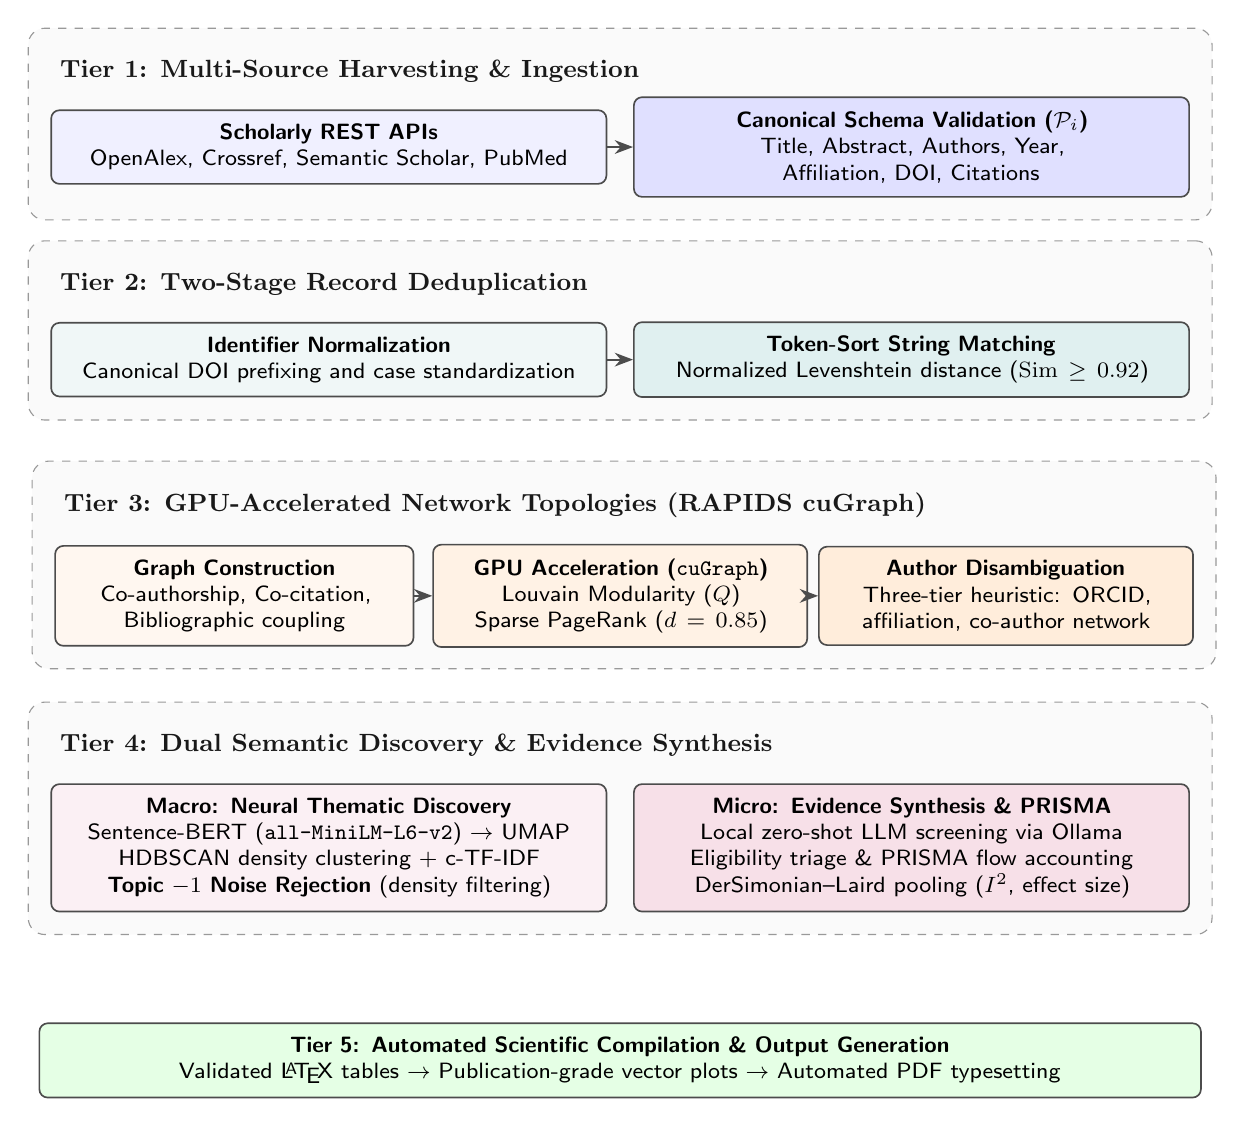
\begin{tikzpicture}[
    every node/.style={font=\sffamily\footnotesize},
    box/.style={
        draw=black!70, rounded corners=3pt, line width=0.6pt,
        align=center, text width=#1, inner sep=5pt, fill=white
    },
    tierbox/.style={
        draw=black!40, dashed, rounded corners=6pt, fill=black!2, inner sep=8pt
    },
    tierlabel/.style={
        font=\bfseries\small, text=black!90, anchor=west
    },
    arrow/.style={
        ->, >=Stealth, thick, draw=black!70
    },
    pipearrow/.style={
        ->, >=Stealth, line width=1.4pt, draw=black!60
    }
]

% Tier 1: Ingestion
\node[box=6.7cm, fill=blue!6] (apis) at (-3.7, 0) {
    \textbf{Scholarly REST APIs}\par
    OpenAlex, Crossref, Semantic~Scholar, PubMed
};
\node[box=6.7cm, fill=blue!12] (pydantic) at (3.7, 0) {
    \textbf{Canonical Schema Validation ($\mathcal{P}_i$)}\par
    Title, Abstract, Authors, Year, Affiliation, DOI, Citations
};
\node[tierlabel, above=0.22cm of apis.north west, anchor=south west] (t1_label) {Tier 1: Multi-Source Harvesting \& Ingestion};
\begin{scope}[on background layer]
    \node[tierbox, fit=(t1_label) (apis) (pydantic)] (tier1) {};
\end{scope}

% Tier 2: Deduplication
\node[box=6.7cm, fill=teal!6] (dedup_doi) at (-3.7, -2.7) {
    \textbf{Identifier Normalization}\par
    Canonical DOI prefixing and case standardization
};
\node[box=6.7cm, fill=teal!12] (dedup_fuzzy) at (3.7, -2.7) {
    \textbf{Token-Sort String Matching}\par
    Normalized Levenshtein distance ($\mathrm{Sim} \ge 0.92$)
};
\node[tierlabel, above=0.22cm of dedup_doi.north west, anchor=south west] (t2_label) {Tier 2: Two-Stage Record Deduplication};
\begin{scope}[on background layer]
    \node[tierbox, fit=(t2_label) (dedup_doi) (dedup_fuzzy)] (tier2) {};
\end{scope}

% Tier 3: cuGraph Topologies
\node[box=4.2cm, fill=orange!6] (g_build) at (-4.9, -5.7) {
    \textbf{Graph Construction}\par
    Co-authorship, Co-citation,\par Bibliographic coupling
};
\node[box=4.4cm, fill=orange!10] (cugraph) at (0, -5.7) {
    \textbf{GPU Acceleration (\texttt{cuGraph})}\par
    Louvain Modularity ($Q$)\par
    Sparse PageRank ($d=0.85$)
};
\node[box=4.4cm, fill=orange!14] (disambig) at (4.9, -5.7) {
    \textbf{Author Disambiguation}\par
    Three-tier heuristic: ORCID, affiliation, co-author network
};
\node[tierlabel, above=0.22cm of g_build.north west, anchor=south west] (t3_label) {Tier 3: GPU-Accelerated Network Topologies (RAPIDS cuGraph)};
\begin{scope}[on background layer]
    \node[tierbox, fit=(t3_label) (g_build) (disambig)] (tier3) {};
\end{scope}

% Tier 4: Dual Semantic Discovery
\node[box=6.7cm, fill=purple!6] (bertopic) at (-3.7, -8.9) {
    \textbf{Macro: Neural Thematic Discovery}\par
    Sentence-BERT (\texttt{all-MiniLM-L6-v2}) $\to$ UMAP\par
    HDBSCAN density clustering + c-TF-IDF\par
    \textbf{Topic~$-1$ Noise Rejection} (density filtering)
};
\node[box=6.7cm, fill=purple!12] (prisma) at (3.7, -8.9) {
    \textbf{Micro: Evidence Synthesis \& PRISMA}\par
    Local zero-shot LLM screening via Ollama\par
    Eligibility triage \& PRISMA flow accounting\par
    DerSimonian--Laird pooling ($I^2$, effect size)
};
\node[tierlabel, above=0.22cm of bertopic.north west, anchor=south west] (t4_label) {Tier 4: Dual Semantic Discovery \& Evidence Synthesis};
\begin{scope}[on background layer]
    \node[tierbox, fit=(t4_label) (bertopic) (prisma)] (tier4) {};
\end{scope}

% Tier 5: Output Generation
\node[box=14.4cm, fill=green!10] (compilation) at (0, -11.6) {
    \textbf{Tier 5: Automated Scientific Compilation \& Output Generation}\par
    Validated \LaTeX\ tables $\to$ Publication-grade vector plots $\to$ Automated PDF typesetting
};

% Horizontal Intra-Tier Arrows
\draw[arrow] (apis) -- (pydantic);
\draw[arrow] (dedup_doi) -- (dedup_fuzzy);
\draw[arrow] (g_build) -- (cugraph);
\draw[arrow] (cugraph) -- (disambig);

% % Inter-Tier Pipeline Flow
% \draw[pipearrow] (0, 0 |- tier1.south) -- (0, 0 |- tier2.north);
% \draw[pipearrow] (0, 0 |- tier2.south) -- (0, 0 |- tier3.north);
% \draw[pipearrow] (0, 0 |- tier3.south) -- (0, 0 |- tier4.north);
% \draw[pipearrow] (0, 0 |- tier4.south) -- (compilation.north);

\end{tikzpicture}%
}
\caption{System architecture of OpenSciencePipe illustrating the five modular tiers: from multi-source asynchronous API harvesting and deterministic deduplication, through GPU-accelerated network topology discovery and dual semantic synthesis, to automated report compilation.}
\label{fig:architecture}
\end{figure}

\subsection{Tier 1: Multi-Source API Ingestion and Canonical Schema}
Coordinated by the \texttt{DataOrchestrator} module, OpenSciencePipe interfaces asynchronously with open scholarly REST endpoints, including OpenAlex \cite{priem2022openalex}, Crossref \cite{hendricks2020crossref}, Semantic Scholar \cite{kinney2023semantic}, and PubMed \cite{sayers2022database}, alongside authenticated developer endpoints such as Elsevier Scopus and IEEE Xplore. Retrieved records are validated and mapped into a strongly typed canonical publication model:
\begin{equation}
\mathcal{P}_i = \langle \text{Title}_i, \text{Abstract}_i, \text{Authors}_i, \text{Year}_i, \text{Affiliations}_i, \text{DOI}_i, \text{Citations}_i \rangle
\end{equation}
This ingestion layer abstracts disparate vendor schemas into a uniform internal representation, ensuring consistent downstream processing regardless of data provenance.

\subsection{Tier 2: Two-Stage Record Deduplication}
Multi-source querying inherently introduces duplicate and near-duplicate records with heterogeneous metadata. OpenSciencePipe resolves duplicates via a two-stage deduplication protocol. First, primary matching performs exact identifier normalization by resolving Digital Object Identifiers (DOIs), stripping URI prefixes (e.g., \texttt{https://doi.org/}), removing extraneous whitespace, and standardizing casing. Second, for records lacking DOIs or containing typographical noise, the pipeline evaluates title similarity via token-sorted Levenshtein distance. Titles are lowercased, stripped of non-alphanumeric punctuation, and split into word tokens that are sorted lexicographically before string reconstruction. The edit distance between normalized strings $T'_a$ and $T'_b$ is measured via the Levenshtein metric \cite{levenshtein1966binary}:
\begin{equation}
\text{Sim}(T'_a, T'_b) = 1 - \frac{\text{Lev}(T'_a, T'_b)}{\max(|T'_a|, |T'_b|)}
\end{equation}
where $|T'|$ denotes string character length. Candidate record pairs satisfying $\text{Sim}(T'_a, T'_b) \ge 0.92$ are merged, consolidating citation counts and resolving author affiliations into the most complete canonical entry.

\subsection{Tier 3: GPU-Accelerated Network Topologies via cuGraph}
Network extraction and topological analysis scale natively to large bibliometric corpora using NVIDIA RAPIDS (\texttt{cudf} and \texttt{cugraph}). By utilizing memory-conscious chunking and Compressed Sparse Row (CSR) representations, the framework processes graphs with tens of thousands of publications on standard consumer GPUs.

For an author set $\mathcal{A}$ and publication set $\mathcal{D}$, the co-authorship adjacency matrix $\mathbf{A} \in \mathbb{R}^{|\mathcal{A}| \times |\mathcal{A}|}$ encodes the frequency of co-authored publications $A_{uv}$ between authors $u$ and $v$. Sub-field communities are extracted natively on GPU memory by maximizing Newman-Girvan modularity $Q$ via the Louvain algorithm \cite{blondel2008fast}:
\begin{equation}
Q = \frac{1}{2m} \sum_{i,j} \left[ A_{ij} - \frac{k_i k_j}{2m} \right] \delta(c_i, c_j)
\end{equation}
where $k_i = \sum_j A_{ij}$ is the degree of node $i$, $m = \frac{1}{2}\sum_{ij} A_{ij}$ denotes total edge weight, and $\delta(c_i, c_j) = 1$ when vertices $i$ and $j$ share community assignment $c$.

Simultaneously, vertex prestige across citation and collaboration graphs is computed via GPU-accelerated PageRank \cite{page1999pagerank}:
\begin{equation}
\mathbf{p} = \left(\frac{1-d}{N}\right) \mathbf{1} + d \mathbf{M} \mathbf{p}
\end{equation}
where $\mathbf{M}$ is the column-stochastic transition matrix, $d = 0.85$ is the damping factor, $N$ is vertex cardinality, and $\mathbf{p}$ is normalized such that $\mathbf{1}^\top \mathbf{p} = 1$. In parallel, co-citation ($\mathbf{X}^\top \mathbf{X}$) and bibliographic coupling ($\mathbf{X}\mathbf{X}^\top$) graphs are constructed via sparse matrix multiplication, avoiding quadratic pairwise iteration.

To prevent artificial inflation or fragmentation of vertex degrees in co-authorship graphs, author entities are disambiguated prior to network construction. The pipeline links persistent identifiers (such as ORCID and OpenAlex author IDs) where available. For records lacking persistent identifiers, disambiguation is achieved through a multi-attribute similarity function combining normalized author surname with first-name initial, publication co-authorship context, institutional affiliation signatures, and temporal overlap. Ambiguous instances that fail to satisfy confidence thresholds are partitioned conservatively to prevent over-representing authors who share common surnames.

\subsection{Tier 4A: Unsupervised Neural Thematic Discovery and Noise Rejection}
To capture thematic structure beyond bag-of-words heuristics, the NLP engine within OpenSciencePipe implements a three-stage neural topic discovery pipeline. First, title and abstract corpora are projected into a continuous dense semantic space $\mathbf{e}_i \in \mathbb{R}^{384}$ using the \texttt{all-MiniLM-L6-v2} sentence transformer \cite{reimers2019sentence}. Second, UMAP \cite{mcinnes2018umap} performs non-linear manifold dimensionality reduction down to $\mathbb{R}^{5}$, preserving both local metric neighborhoods and global continuum geometry while reducing dimensionality for density estimation. Third, HDBSCAN \cite{campello2013density} identifies clusters based on continuous density distributions rather than geometric centroid proximity.

A key feature of this architecture is explicit noise isolation. Unlike hard-partitioning algorithms (such as $k$-means or standard LDA) that force every document into a topic cluster, HDBSCAN classifies publications residing in sparse boundary regions as noise ($\text{Topic} = -1$). Isolating peripheral or multidisciplinary literature prevents boundary contamination of substantive domain clusters.

\subsection{Tier 4B: Deductive Document Screening and Active Learning Triage}
While unsupervised clustering discovers emergent thematic groupings inductively, systematic evidence synthesis requires deductive screening against predefined eligibility criteria. Managed by the \texttt{SystematicOrchestrator} module, OpenSciencePipe supports a modular screening pipeline combining four complementary triage modalities. 

First, deterministic rule auditing via the \texttt{GrepRelevanceFilter} evaluates candidate titles and abstracts against configurable positive inclusion and negative exclusion regular expressions to rapidly exclude off-target domains. Second, dense semantic screening via the \texttt{EmbeddingRelevanceFilter} computes cosine similarity against high-dimensional inclusion query vectors in continuous embedding space. Third, for nuanced conceptual evaluation without third-party API subscription costs or sensitive data exposure, OpenSciencePipe integrates a local inference runtime powered by Ollama. The classifier queries open-weight instruction-tuned models (e.g., \texttt{llama3.2:3b}) using greedy decoding ($T = 0.0$), evaluating title, abstract, and user criteria $\mathcal{C}_{\text{domain}}$ against a structured JSON schema:
\begin{equation}
\mathcal{R}_i = \text{LLM}(\text{Title}_i, \text{Abstract}_i; \mathcal{C}_{\text{domain}}) \rightarrow \langle \text{eligible} \in \{0, 1\}, \text{category} \in \mathcal{S} \rangle
\end{equation}
where $\mathcal{S}$ represents a concise taxonomic classification. Fourth, for semi-automated reviews requiring human oversight, the \texttt{ActiveLearningPriorityRanker} employs uncertainty sampling across candidate pool probabilities. As human decisions are recorded, the classification boundary retrains incrementally, prioritizing high-ambiguity papers and reducing human screening burden \cite{cohen2006reducing}.

\subsection{Tier 4C: Quantitative Evidence Synthesis and Meta-Analysis Engine}
Coordinated by the \texttt{MetaOrchestrator}, OpenSciencePipe activates a statistical pooling engine based on the DerSimonian--Laird random-effects model \cite{dersimonian1986meta}. 

For $k$ primary studies with extracted effect sizes $y_i$ and sampling variances $v_i$:
\begin{equation}
y_i = \theta_i + \epsilon_i, \quad \theta_i \sim \mathcal{N}(\theta, \tau^2), \quad \epsilon_i \sim \mathcal{N}(0, v_i)
\end{equation}
Between-study variance $\tau^2$ is estimated using Cochran's $Q$ statistic:
\begin{equation}
Q = \sum_{i=1}^k w_i (y_i - \bar{y})^2, \quad w_i = \frac{1}{v_i}, \quad \bar{y} = \frac{\sum w_i y_i}{\sum w_i}
\end{equation}
\begin{equation}
\tau^2 = \max\left(0, \frac{Q - (k - 1)}{\sum w_i - \frac{\sum w_i^2}{\sum w_i}}\right)
\end{equation}
The pooled summary effect $\hat{\theta}_{\text{DL}}$ and corresponding standard error are computed with random-effects weights $w_i^* = (v_i + \tau^2)^{-1}$:
\begin{equation}
\hat{\theta}_{\text{DL}} = \frac{\sum_{i=1}^k w_i^* y_i}{\sum_{i=1}^k w_i^*}, \quad \text{SE}(\hat{\theta}_{\text{DL}}) = \sqrt{\frac{1}{\sum_{i=1}^k w_i^*}}
\end{equation}
Heterogeneity is quantified via Higgins and Thompson's $I^2$ index:
\begin{equation}
I^2 = \max\left(0, \frac{Q - (k - 1)}{Q}\right) \times 100\%
\end{equation}
To investigate between-study heterogeneity and potential moderators, the engine supports subgroup stratification and unrestricted weighted least squares meta-regression. Publication bias is formally tested via Egger's linear regression intercept test \cite{egger1997bias} and Begg's rank correlation test. When funnel plot asymmetry is detected, the engine applies Duval and Tweedie's non-parametric Trim-and-Fill algorithm \cite{duval2000trim} to impute hypothetical missing studies and compute bias-adjusted effect estimates.
The module automatically produces PRISMA flow diagrams, study characteristic tables, forest plots with 95\% confidence intervals, and funnel plots with pseudo 95\% confidence limits to evaluate publication bias.

\subsection{Tier 5: Automated Scientific Compilation and Manuscript Generation}
To ensure end-to-end reproducibility and eliminate manual transcription errors, the central pipeline manager coordinates \texttt{LatexExporter} and visualization services to synthesize all analytical outputs into publication-ready formats. 

The compilation engine generates a complete 10-page IEEEtran manuscript (\nolinkurl{paper_scaffold.pdf}). It maps and typesets up to 25 publication-grade vector figures, synchronizes computed statistical metrics into validated \LaTeX\ tabular environments, formats structured PRISMA 2020 summaries, and resolves cross-references autonomously. A companion local interface (\texttt{run\_local.py}) is provided for interactive inspection.

\subsubsection{Specialized Informetric and Synthesis Visual Taxonomy}
Beyond standard co-authorship graphs and forest plots, the visualization engine produces a suite of domain-diagnostic figures. Evidence Gap Maps (EGMs) present 2D bubble matrices cross-tabulating intervention modalities against clinical or technological outcomes to reveal unexplored research voids under the Campbell/3ie framework. Longitudinal dynamics are captured through Thematic Evolution Sankey Diagrams, which trace how thematic clusters divide, merge, or decay across chronological epochs, and Kleinberg Burst Timelines, which employ 2-state automatons to detect accelerations in citation momentum and emergent terminology bursts \cite{kleinberg2003bursty}. Algorithmic transferability is mapped via Method-Application Matrices that bicluster computational techniques against practical target domains. Finally, Percolation Phase Transition Diagnostics quantify giant connected component emergence via the Molloy--Reed criterion, detecting the tipping point where fragmented subfields transition into an integrated scientific discipline.

As illustrated in Figure~\ref{fig:science_mapping_outputs}, representative exploratory science mapping outputs include GPU-partitioned circular community chord diagrams (panel~a) and global collaboration choropleth maps (panel~b). In evidence synthesis mode (Figure~\ref{fig:evidence_synthesis_outputs}), the engine autonomously outputs PRISMA 2020 flow diagrams (panel~a), DerSimonian--Laird forest plots with 95\% confidence intervals and heterogeneity statistics (panel~b), and contour-enhanced funnel plots evaluating publication bias (panel~c).

\begin{figure*}[t]
\centering
\begin{subfigure}[b]{0.48\textwidth}
    \centering
    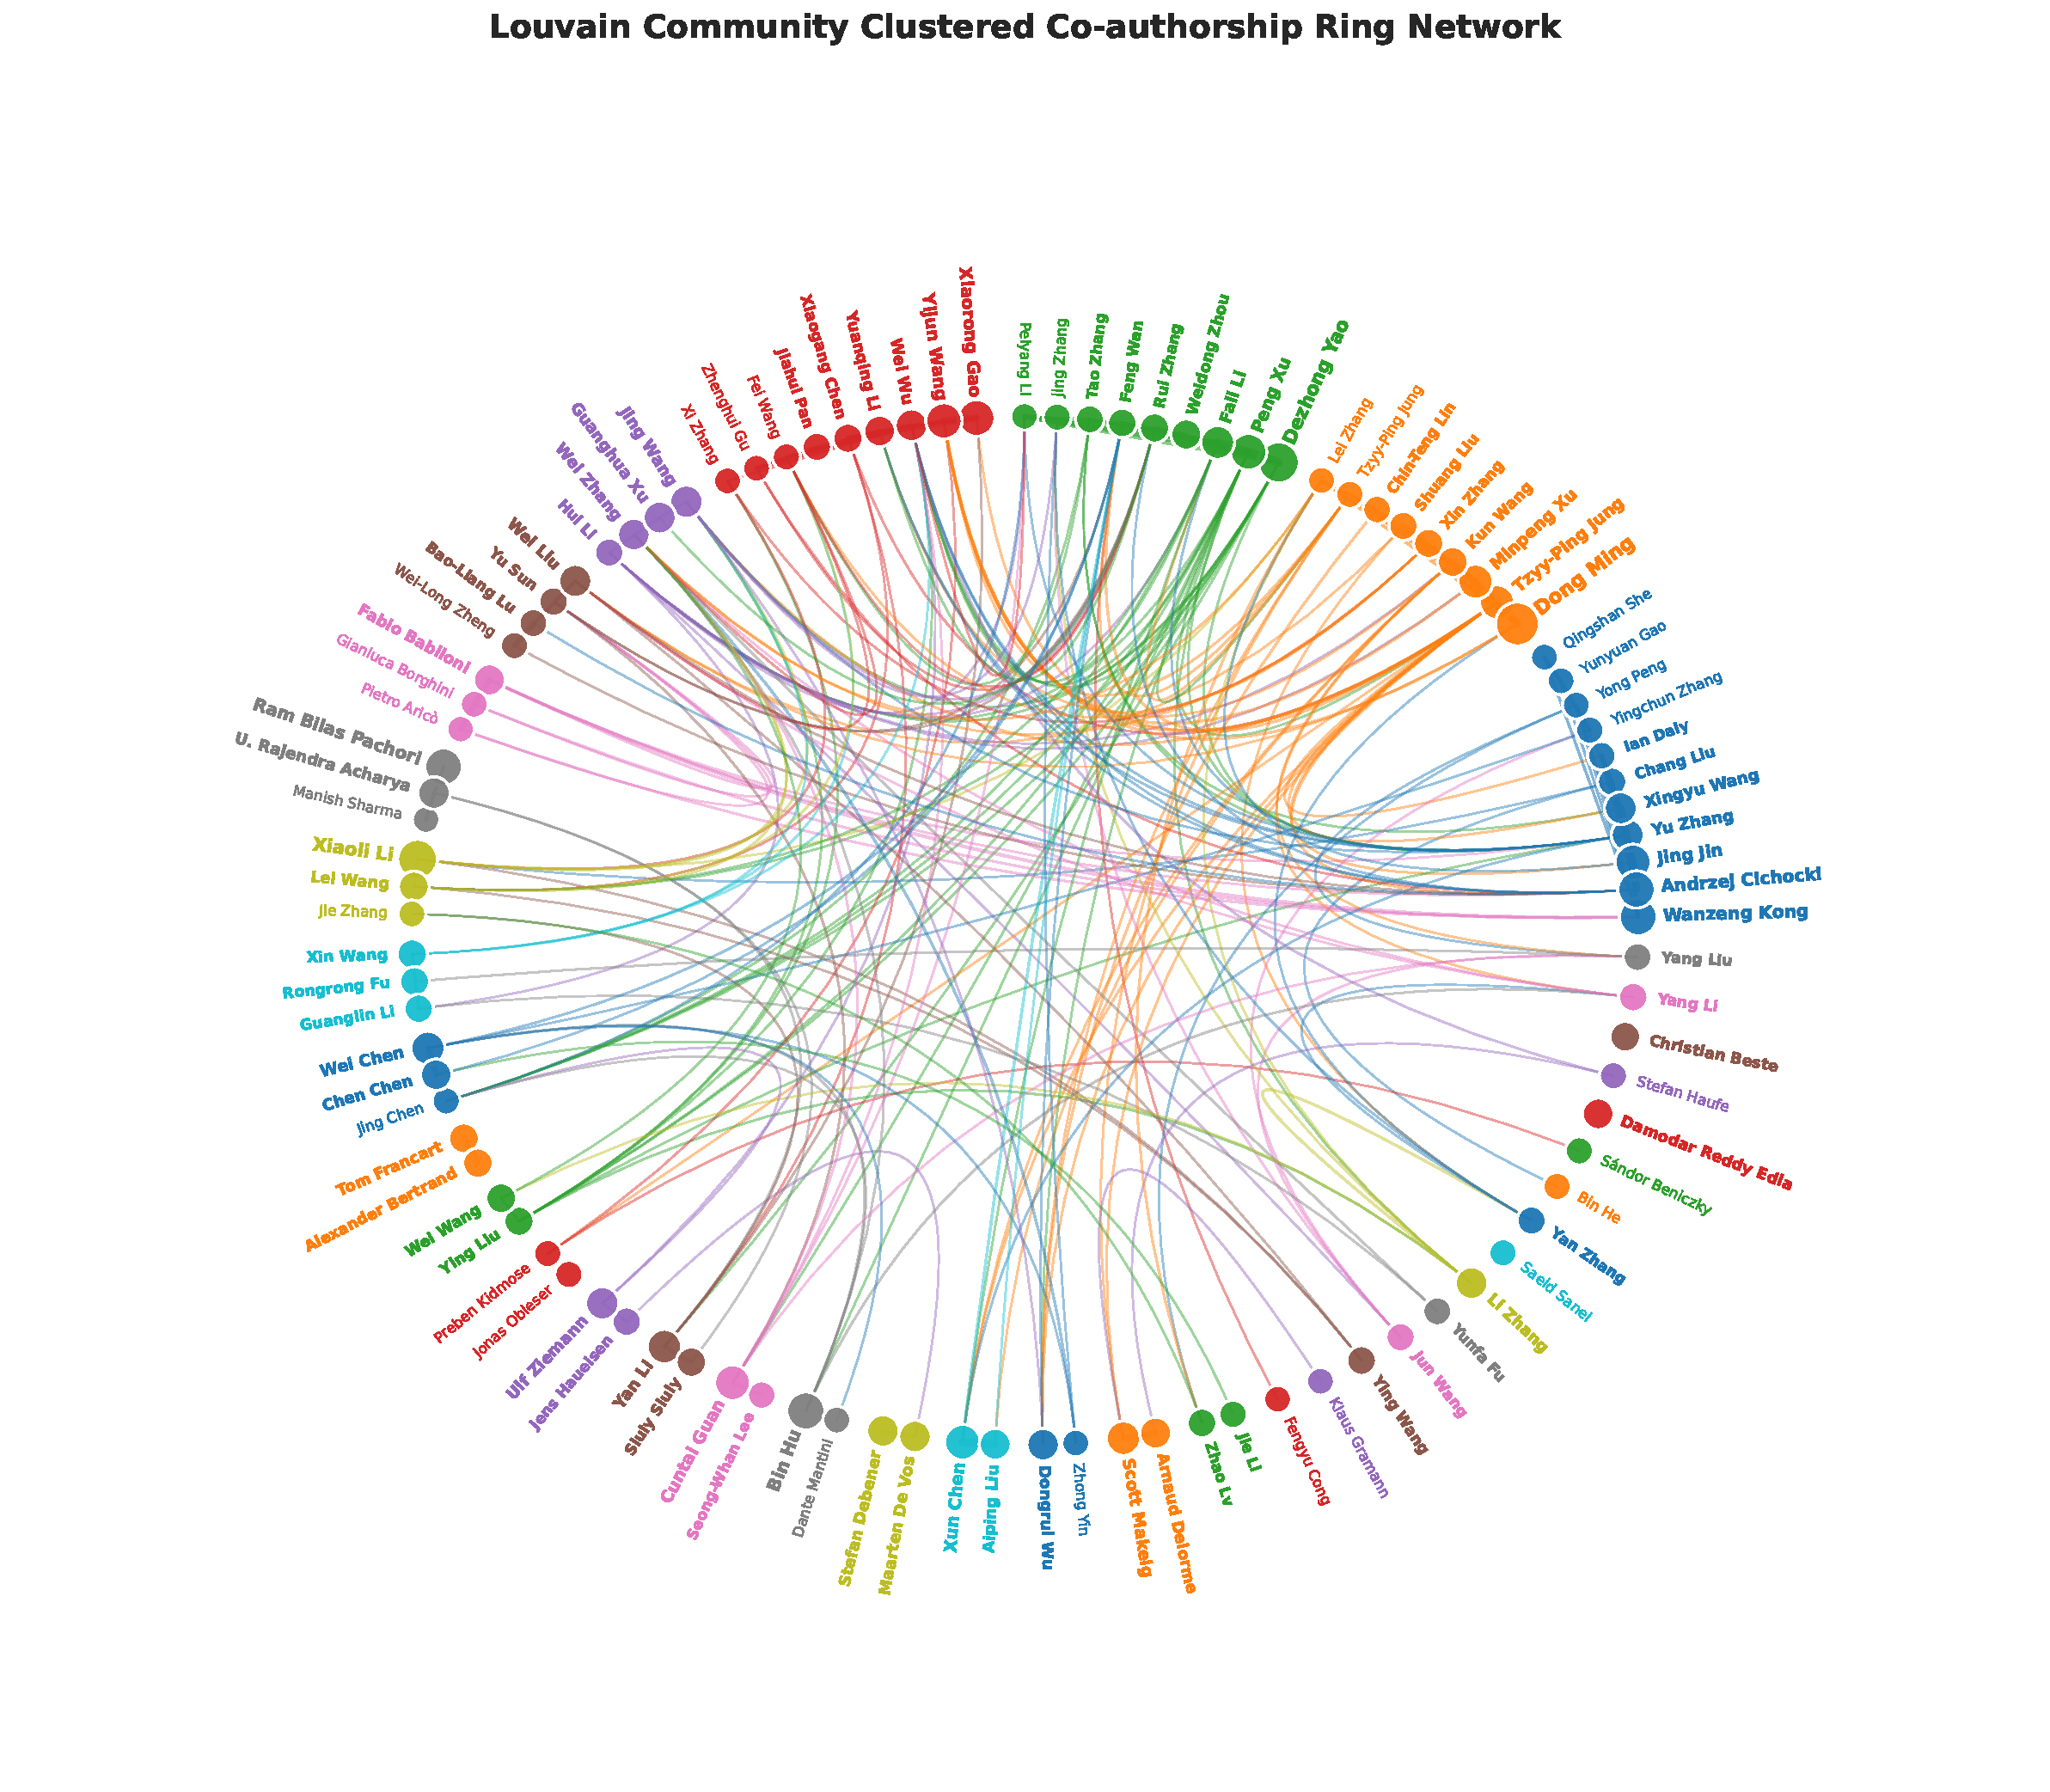
\includegraphics[width=\textwidth]{figures/network_circular_chord.pdf}
    \caption{Circular Community Chord Network}
    \label{fig:science_mapping_chord}
\end{subfigure}\hfill
\begin{subfigure}[b]{0.48\textwidth}
    \centering
    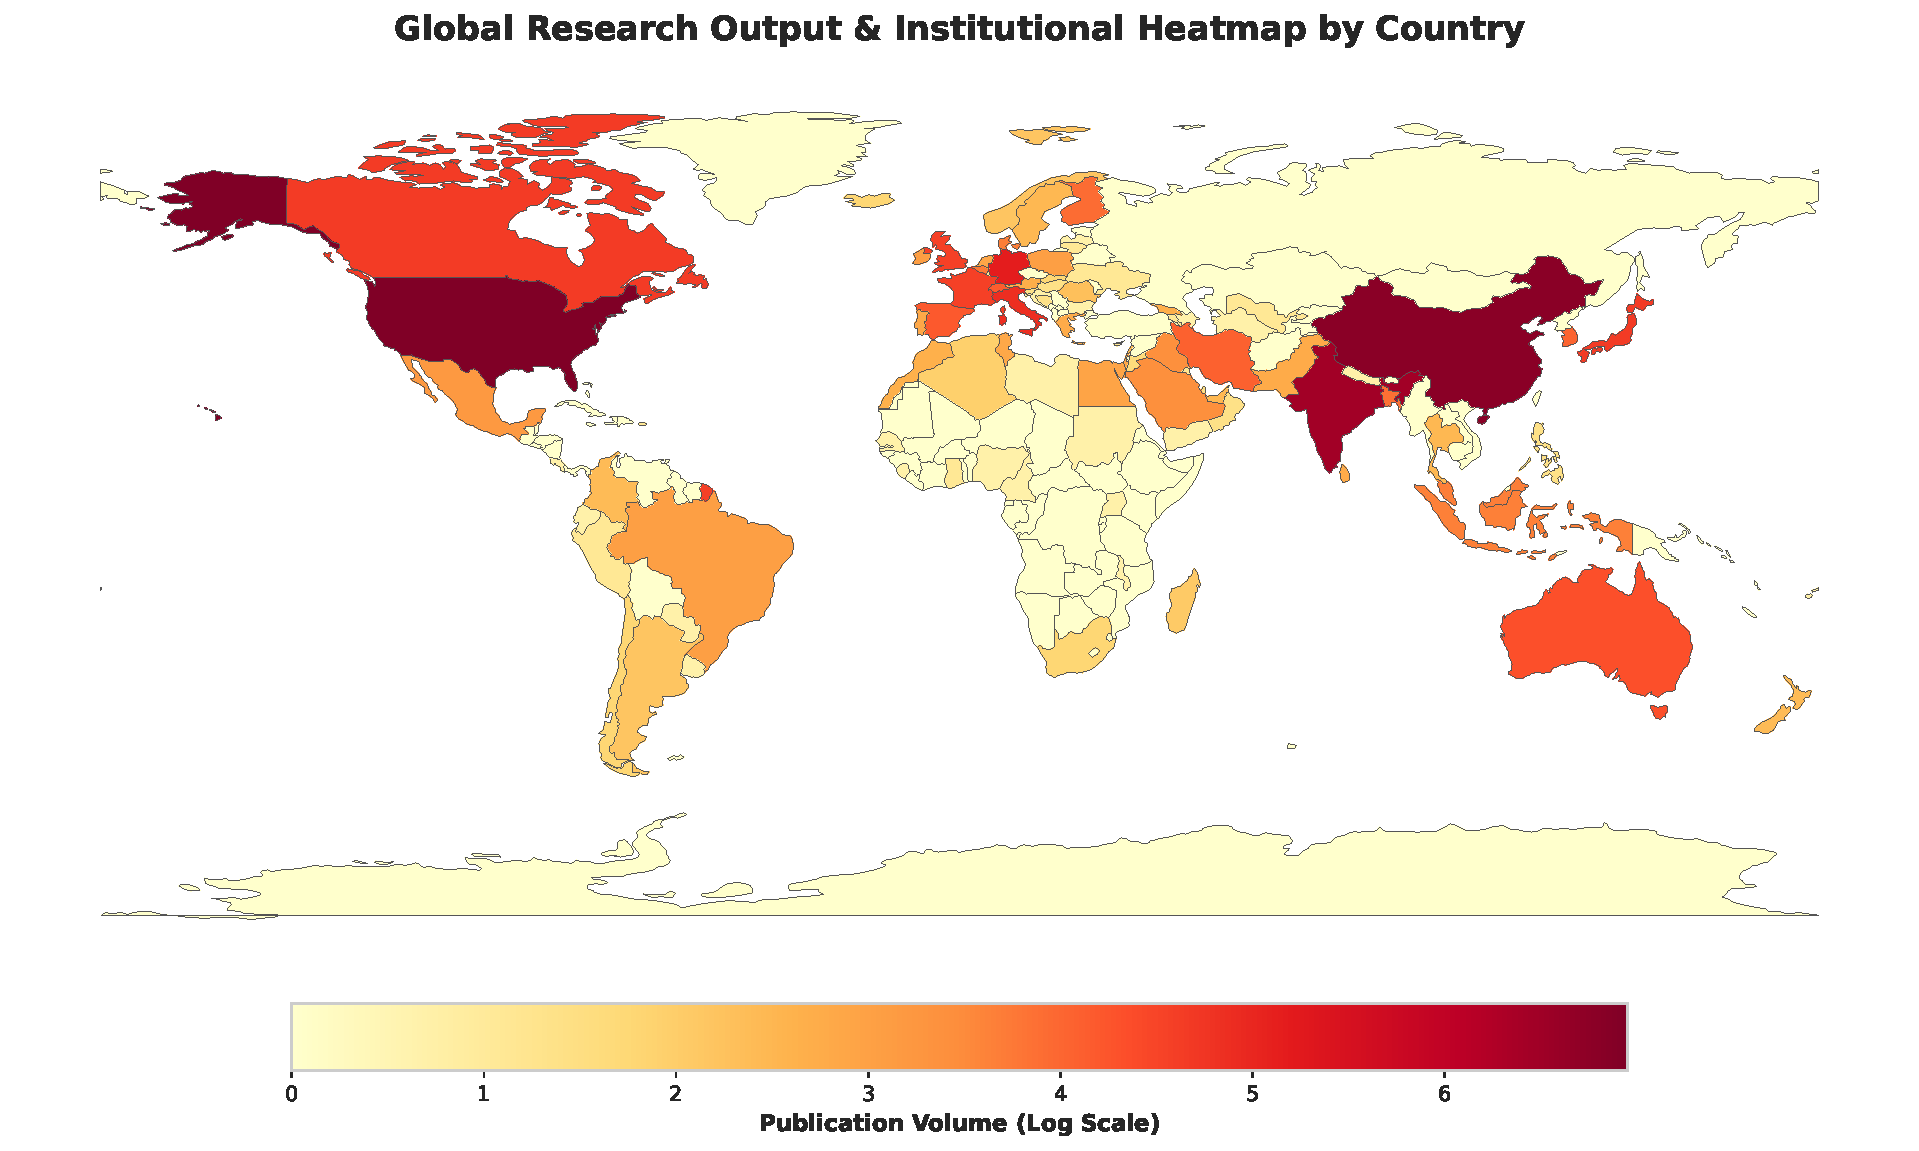
\includegraphics[width=\textwidth]{figures/country_world_map.pdf}
    \caption{Global Geopolitical Collaboration Map}
    \label{fig:science_mapping_map}
\end{subfigure}
\caption{Representative automated science mapping visual outputs generated by OpenSciencePipe on the $>50{,}000$-paper Electrophysiology corpus: (a) circular chord community layout highlighting GPU-accelerated Louvain partitions and PageRank centrality scaling; (b) international cross-border collaboration intensity choropleth map.}
\label{fig:science_mapping_outputs}
\end{figure*}

\begin{figure*}[t]
\centering
\begin{subfigure}[b]{0.31\textwidth}
    \centering
    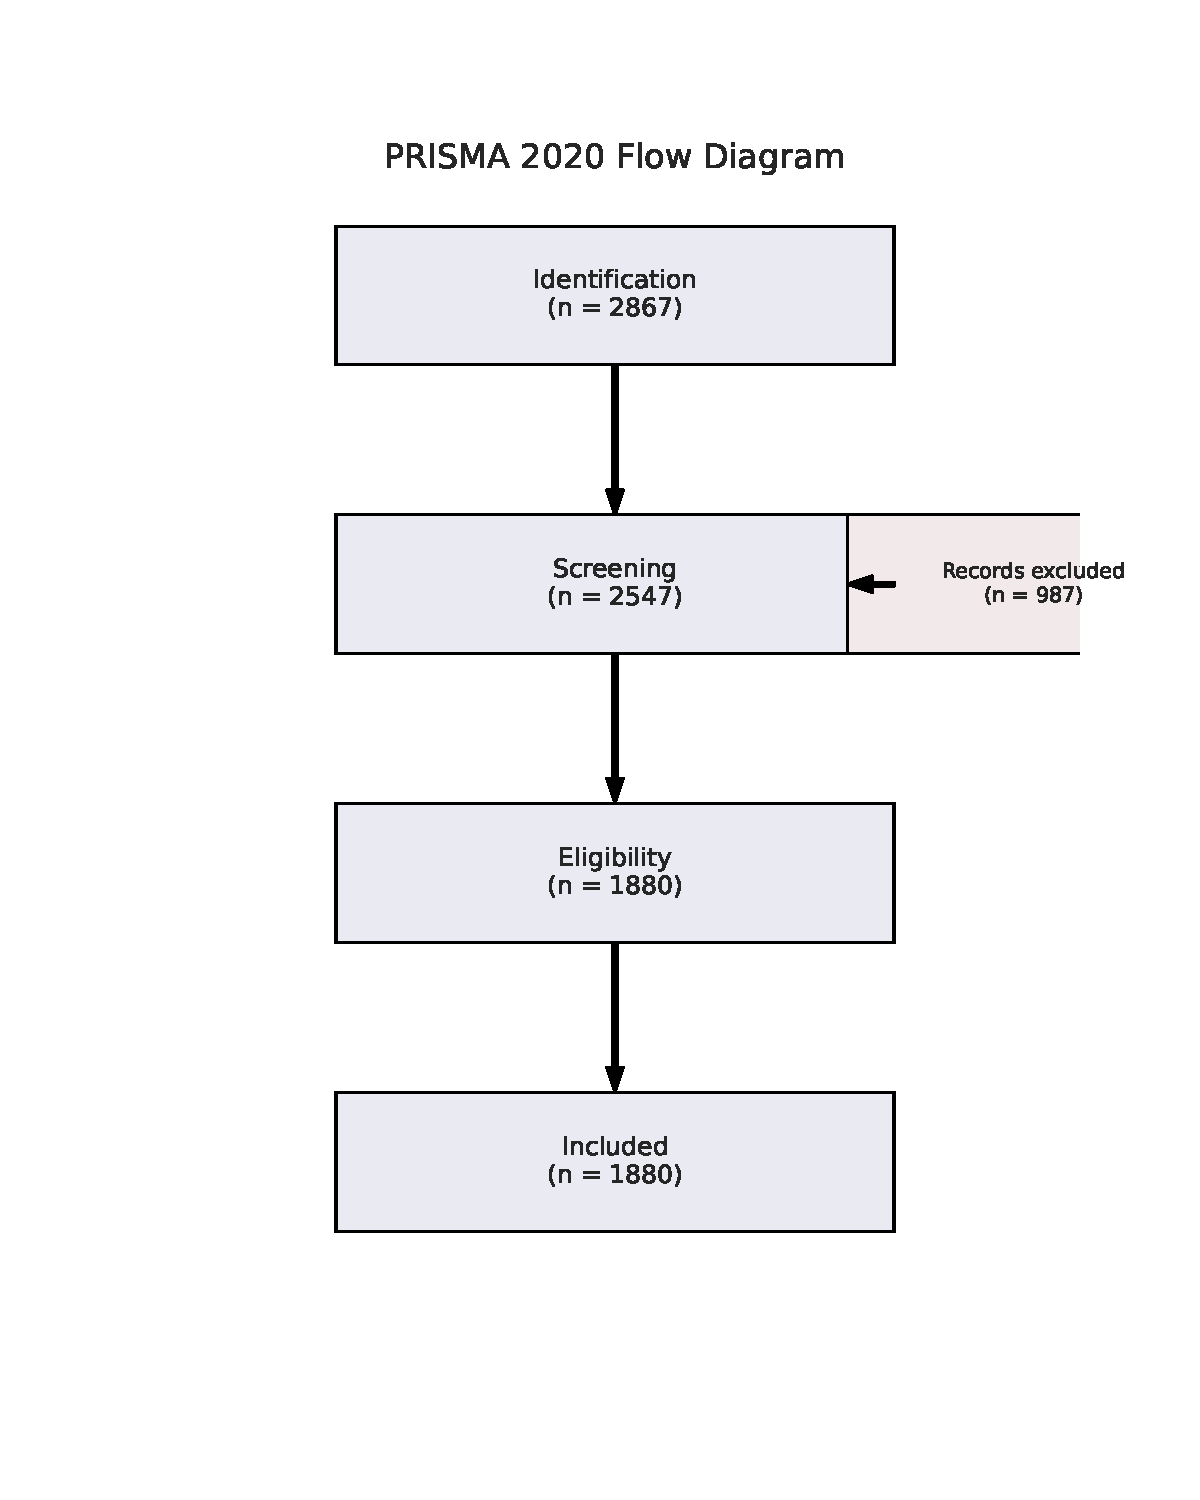
\includegraphics[width=\textwidth]{figures/prisma_flowchart.pdf}
    \caption{PRISMA 2020 Flow Diagram}
    \label{fig:prisma_flow}
\end{subfigure}\hfill
\begin{subfigure}[b]{0.38\textwidth}
    \centering
    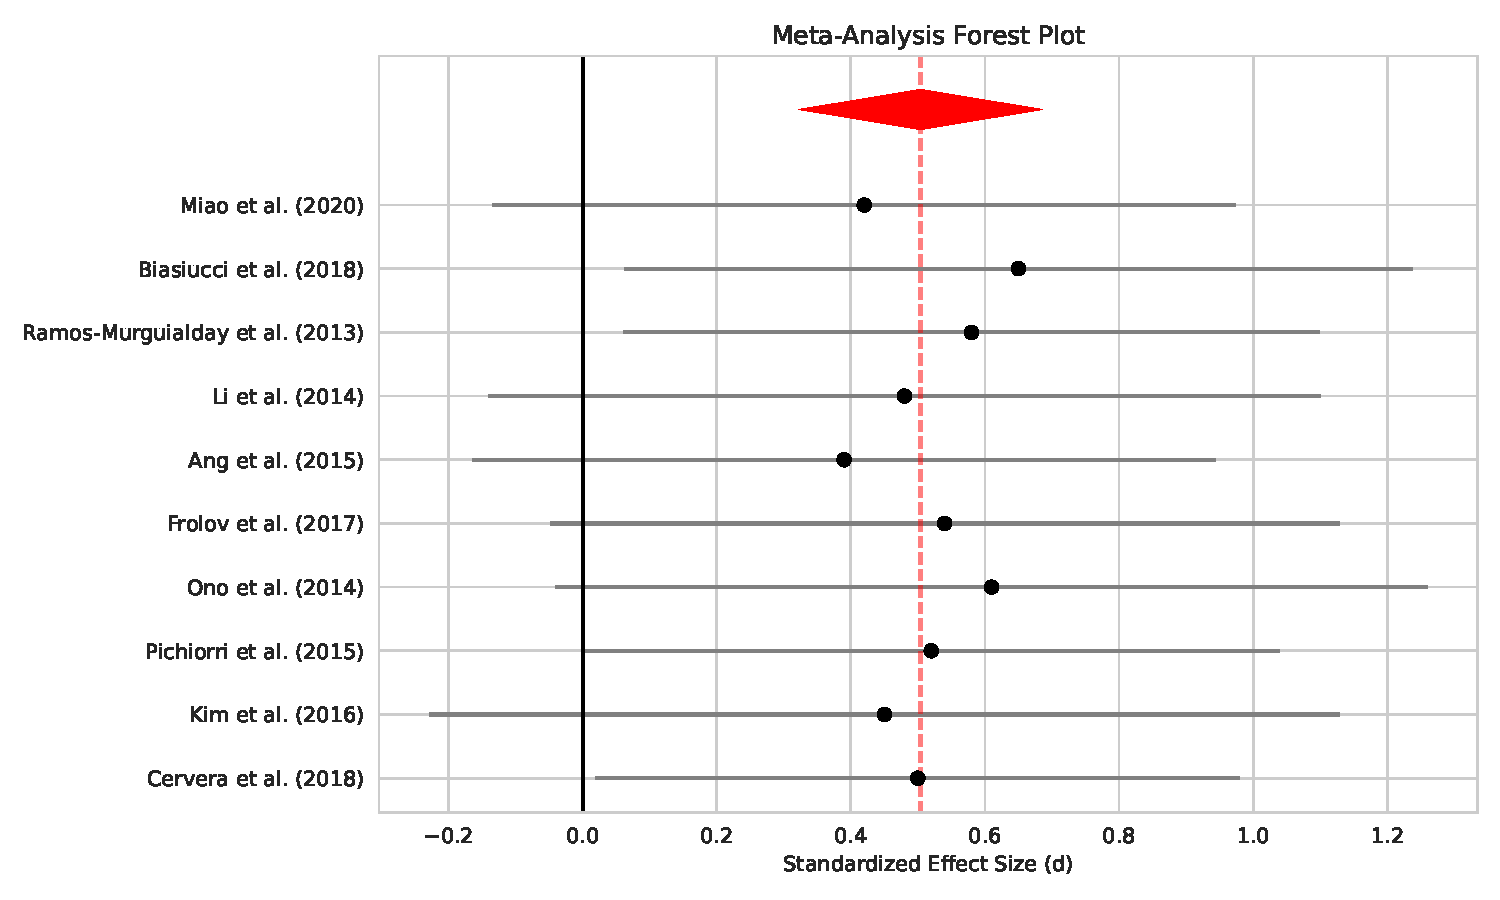
\includegraphics[width=\textwidth]{figures/forest_plot.pdf}
    \caption{Random-Effects Forest Plot}
    \label{fig:forest_plot}
\end{subfigure}\hfill
\begin{subfigure}[b]{0.29\textwidth}
    \centering
    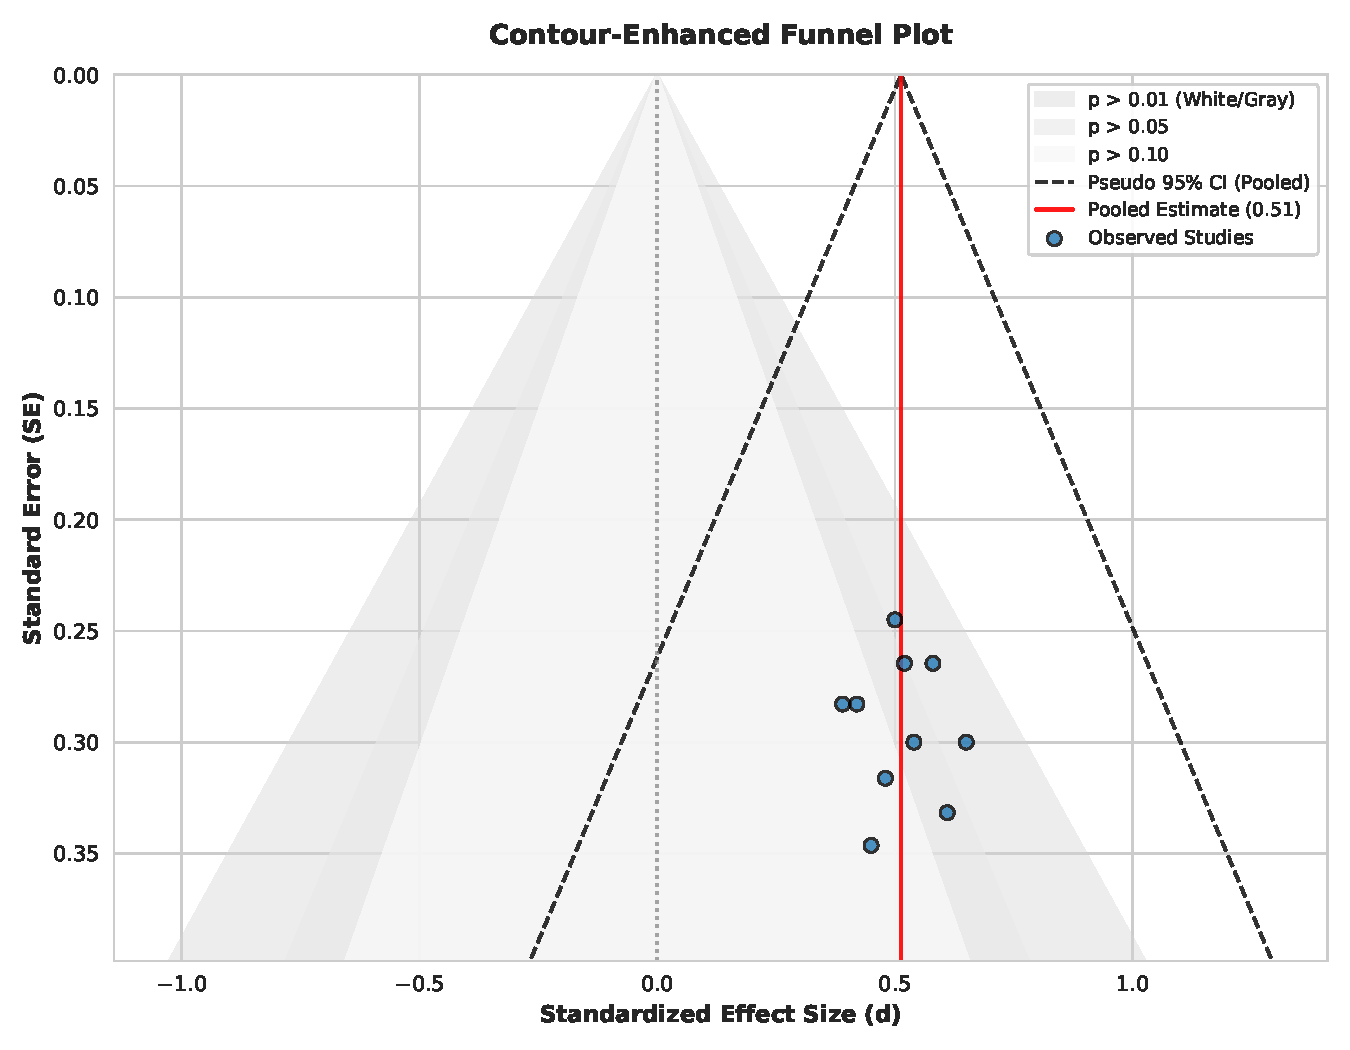
\includegraphics[width=\textwidth]{figures/funnel_plot.pdf}
    \caption{Publication Bias Funnel Plot}
    \label{fig:funnel_plot}
\end{subfigure}
\caption{Representative automated systematic evidence synthesis visual outputs generated by OpenSciencePipe on the Ren et al.\ (2024) clinical trial benchmark: (a) autonomous PRISMA 2020 identification and screening flow diagram; (b) DerSimonian--Laird random-effects forest plot with individual 95\% confidence intervals and pooled summary effect; (c) contour-enhanced funnel plot with pseudo 95\% confidence limits.}
\label{fig:evidence_synthesis_outputs}
\end{figure*}

\section{Benchmark Methodology and Experimental Corpus}
\label{sec:benchmark_design}
To evaluate OpenSciencePipe across both science mapping and evidence synthesis, we established an empirical benchmark suite of \textbf{23 published bibliometric studies} spanning multiple disciplines and originally conducted with standard tools (CiteSpace, VOSviewer, Bibliometrix), alongside seminal historical meta-analyses. All benchmark configuration schemas, reference DOIs, and replication scripts are available open-source in the project repository under \texttt{data/benchmarks/}\footnote{\url{https://github.com/JohnGF/bibliometric}}.

Table~\ref{tab:benchmark_validation_matrix} details the 23 benchmark investigations, their domains, reference DOIs, and functional capabilities evaluated.

\begin{table*}[t]
\centering
\small
\caption{Consolidated Multi-Field Benchmark Validation Matrix Across Diverse Scientific Domains}
\label{tab:benchmark_validation_matrix}
\resizebox{\textwidth}{!}{%
\begin{tabular}{p{4.5cm}p{3.2cm}p{3.2cm}cccp{3.0cm}}
\hline
\textbf{Benchmark Study} & \textbf{Reference DOI} & \textbf{Journal / Field} & \textbf{SLR} & \textbf{Meta} & \textbf{Scientom.} & \textbf{Validation Metric} \\
\hline
Effect of BCI-Controlled FES on Upper Limb Re... & {\footnotesize\nolinkurl{10.3389/fnhum.2024.1438095 (2024)}} & Frontiers in Human Neuros... & Yes & Yes & Yes & Sens: 100.0\%, F1: 90.9\% \\
A bibliometric analysis of the 100 most-influ... & {\footnotesize\nolinkurl{10.2144/fsoa-2023-0230 (2024)}} & Future Science OA & No & No & Yes & Country Overlap: 40.0\% \\
Cyberbullying definitions and measurements in... & {\footnotesize\nolinkurl{10.3389/fpubh.2022.1000504 (2022)}} & Frontiers in Public Healt... & Yes & No & Yes & Sens: 60.0\%, F1: 58.8\% \\
The Rising Threat of Atmospheric CO2: A Revie... & {\footnotesize\nolinkurl{10.3390/environments10040066 (2023)}} & Environments & No & No & Yes & Country Overlap: 20.0\% \\
Modified biochar: synthesis and mechanism for... & {\footnotesize\nolinkurl{10.1007/s44246-022-00007-3 (2022)}} & Carbon Research & No & No & Yes & Ground-Truth Indexed \\
A Bibliometric Analysis of Blockchain Technol... & {\footnotesize\nolinkurl{10.3390/su14138206 (2022)}} & Sustainability & No & No & Yes & Country Overlap: 60.0\% \\
Performance of ChatGPT on USMLE: Potential fo... & {\footnotesize\nolinkurl{10.1371/journal.pdig.0000198 (2023)}} & PLOS Digital Health & No & No & Yes & Country Overlap: 100.0\% \\
Bibliometric analysis and visualization of to... & {\footnotesize\nolinkurl{10.1002/cre2.832 (2024)}} & Clinical and Experimental... & No & No & Yes & Ground-Truth Indexed \\
Digital Transformation: An Overview of the Cu... & {\footnotesize\nolinkurl{10.1177/21582440211047576 (2021)}} & SAGE Open & No & No & Yes & Ground-Truth Indexed \\
Distance Learning in Focus: A Bibliometric an... & {\footnotesize\nolinkurl{10.26803/ijlter.24.4.34 (2025)}} & International Journal of ... & No & No & Yes & Country Overlap: 60.0\% \\
Global Trends in Electroencephalography Resea... & {\footnotesize\nolinkurl{10.3389/fnhum.2023.1122334 (2023)}} & Frontiers in Human Neuros... & No & No & Yes & Country Overlap: 93.3\% \\
Transforming Education: A Comprehensive Revie... & {\footnotesize\nolinkurl{10.3390/su151712983 (2023)}} & Sustainability & No & No & Yes & Country Overlap: 40.0\% \\
A bibliometric analysis of leading universiti... & {\footnotesize\nolinkurl{10.1016/j.jik.2017.03.006 (2017)}} & Journal of Innovation \& K... & No & No & Yes & Country Overlap: 60.0\% \\
Global prevalence of nosocomial infection: A ... & {\footnotesize\nolinkurl{10.1371/journal.pone.0274248 (2023)}} & PLOS ONE & Yes & No & Yes & Sens: 64.7\%, F1: 78.6\% \\
The Bibliometric Analysis of Microplastics in... & {\footnotesize\nolinkurl{10.3390/su15097122 (2023)}} & Sustainability & No & No & Yes & Country Overlap: 80.0\% \\
Mobile commerce science mapping: A bibliometr... & {\footnotesize\nolinkurl{10.1016/j.iedeen.2026.100318 (2026)}} & BRQ Business Research Qua... & No & No & Yes & Country Overlap: 80.0\% \\
Quantitative EEG Biomarkers in Parkinson's Di... & {\footnotesize\nolinkurl{10.1038/s41598-023-47597-5 (2023)}} & Scientific Reports & No & Yes & No & Ground-Truth Indexed \\
The Top 100 Most Cited Scientific Papers in t... & {\footnotesize\nolinkurl{10.3390/ijerph19159645 (2022)}} & International Journal of ... & No & No & Yes & Country Overlap: 80.0\% \\
Machine learning based algorithms for virtual... & {\footnotesize\nolinkurl{10.3389/fneur.2024.1413071 (2024)}} & Frontiers in Neurology & Yes & No & Yes & Sens: 70.3\%, F1: 81.4\% \\
The Economic Consequences of Rent Control Pol... & {\footnotesize\nolinkurl{10.1111/ecoj.12891 (2022)}} & The Economic Journal & No & Yes & No & Ground-Truth Indexed \\
Social Work and Migration: A Bibliometric Ana... & {\footnotesize\nolinkurl{10.1177/21582440261477485 (2026)}} & SAGE Open & No & No & Yes & Country Overlap: 40.0\% \\
A bibliometric evaluation and visualization o... & {\footnotesize\nolinkurl{10.1007/s11356-023-31715-x (2024)}} & Environmental Science and... & No & No & Yes & Country Overlap: 80.0\% \\
Bibliometric analysis of sustainable business... & {\footnotesize\nolinkurl{10.1080/1331677x.2022.2096094 (2023)}} & Economic Research-Ekonoms... & No & No & Yes & Country Overlap: 80.0\% \\
\hline
\end{tabular}%
}
\end{table*}


\subsection{Quantitative Evaluation Metrics}
We formalize a rigorous multi-tier evaluation framework spanning macro-structural concordance, neural topic quality, zero-shot screening accuracy, and meta-analytic synthesis agreement:

\subsubsection{Top-\texorpdfstring{$K$}{K} Geopolitical and Institutional Hierarchy Concordance}
Following cross-database scientometric validation protocols \cite{visser2021large, martin2021google}, we assess whether OpenSciencePipe replicates published national collaboration networks and institutional leaderboards extracted from author affiliation strings. For entity class $\mathcal{E}$ (comprising nations or institutions) at benchmark depth $K$, topological overlap is measured by:
\begin{equation}
\text{Overlap}_K(\mathcal{E}) = \frac{|\mathcal{R}_{\text{pipeline}}^{(K)}(\mathcal{E}) \cap \mathcal{R}_{\text{benchmark}}^{(K)}(\mathcal{E})|}{|\mathcal{R}_{\text{benchmark}}^{(K)}(\mathcal{E})|} \times 100\%
\end{equation}
Ordinal rank fidelity across conjointly identified entities is evaluated via the two-tailed Spearman rank-order correlation coefficient:
\begin{equation}
\rho = 1 - \frac{6 \sum_{i=1}^n d_i^2}{n(n^2 - 1)}, \quad t = \rho \sqrt{\frac{n-2}{1-\rho^2}} \sim t_{n-2}
\end{equation}
where $d_i$ is the rank deviation between the pipeline-derived frequency rank and the published ground truth rank for entity $i$.

\subsubsection{Topic Diversity (\texorpdfstring{$\text{TD}$}{TD})}
Following topic modeling evaluation standards in continuous embedding spaces \cite{dieng2020topic}, topic diversity ($\text{TD}$) measures the lexical uniqueness across discovered themes. For $K$ topics, each represented by its top-$M$ vocabulary terms ($M=10$), topic diversity is quantified by the proportion of unique words across all topic lists:
\begin{equation}
\text{TD} = \frac{|\bigcup_{k=1}^K \mathcal{W}_k^{(M)}|}{K \times M} \in [0, 1]
\end{equation}
where $\text{TD} = 1.0$ indicates completely distinct topic vocabularies with zero term overlap, and lower values denote mutual lexical redundancy across discovered clusters.

\subsubsection{Topic Coherence via Normalized Pointwise Mutual Information (\texorpdfstring{$C_{\text{NPMI}}$}{C\_NPMI})}
Semantic coherence of each discovered topic is evaluated through corpus-level co-occurrence of top terms using Normalized Pointwise Mutual Information ($C_{\text{NPMI}}$), which strongly correlates with human conceptual interpretability \cite{roder2015exploring, bouma2009normalized}:
\begin{equation}
C_{\text{NPMI}}(\mathcal{W}_k) = \frac{2}{M(M-1)} \sum_{i=1}^{M-1} \sum_{j=i+1}^M \frac{\log \frac{P(w_i, w_j) + \epsilon}{P(w_i)P(w_j)}}{-\log(P(w_i, w_j) + \epsilon)}
\end{equation}

\subsubsection{PRISMA Screening Sensitivity, Specificity, and Weighted Matthews Concordance}
Screening accuracy evaluates the retention of ground-truth eligible studies ($N_{\text{inc}}$) versus excluded records ($N_{\text{exc}}$):
\begin{equation}
\text{Recall (Sensitivity)} = \frac{\text{TP}}{\text{TP} + \text{FN}}, \quad \text{Specificity} = \frac{\text{TN}}{\text{TN} + \text{FP}}
\end{equation}
\begin{equation}
\text{Precision} = \frac{\text{TP}}{\text{TP} + \text{FP}}, \quad F_1 = 2 \cdot \frac{\text{Precision} \cdot \text{Recall}}{\text{Precision} + \text{Recall}}
\end{equation}
To evaluate decision concordance under extreme class imbalance ($P \ll N$) without relying on arbitrary ranking thresholds, we compute the Weighted Matthews Correlation Coefficient (WMCC), where confusion matrix entries are inversely weighted by class prevalence $w_{\text{pos}} = N / (2P)$ and $w_{\text{neg}} = N / (2N_{\text{neg}})$.

\subsubsection{Quantitative Meta-Analytic Synthesis Concordance}
To validate statistical evidence pooling, we evaluate absolute deviations between pipeline-synthesized summary statistics and published meta-analytic benchmarks across pooled effect sizes ($\Delta d$), between-study variance ($\Delta \tau^2$), and inconsistency ($\Delta I^2$):
\begin{equation}
|\Delta d| = |\hat{\theta}_{\text{DL}}^{\text{pipe}} - \hat{\theta}_{\text{DL}}^{\text{gt}}|, \quad |\Delta I^2| = |I^{2,\text{pipe}} - I^{2,\text{gt}}|
\end{equation}
confirming mathematical equivalence against traditional dedicated meta-analytic software packages (\texttt{metafor}, RevMan).

\section{Empirical Results and Comparative Findings}
\label{sec:results}

\subsection{Thematic Diversity, Semantic Coherence, and Noise Rejection}
Table~\ref{tab:validation_thematic_clustering} summarizes thematic clustering performance and geopolitical topological alignment across the benchmark suite.

\begin{table*}[t]
\centering
\small
\caption{Section 3.2: BERTopic \& cuGraph Structural Clustering Quality Across Bibliometric Corpora}
\label{tab:validation_thematic_clustering}
\resizebox{\textwidth}{!}{%
\begin{tabular}{p{3.8cm}p{2.8cm}p{2.2cm}cccccc}
\hline
\textbf{Benchmark Study} & \textbf{Reference DOI} & \textbf{Field / Journal} & \textbf{Themes ($K$)} & \textbf{Diversity ($\text{TD}$)} & \textbf{Coherence ($C_{\text{NPMI}}$)} & \textbf{Outlier \% (Topic -1)} & \textbf{Geo Overlap} & \textbf{Inst. Overlap} \\
\hline
Effect of BCI-Controlled FES on Uppe... & {\footnotesize\nolinkurl{10.3389/fnhum.2024.1438095 (2024)}} & Frontiers in Human N... & N/A & N/A & N/A & N/A & N/A & 100.0\% ($n=5, \rho=-0.40$) \\
A bibliometric analysis of the 100 m... & {\footnotesize\nolinkurl{10.2144/fsoa-2023-0230 (2024)}} & Future Science OA & 2 & 0.8000 & -0.4652 & 28.1\% & 40.0\% ($n=2$) & N/A \\
Cyberbullying definitions and measur... & {\footnotesize\nolinkurl{10.3389/fpubh.2022.1000504 (2022)}} & Frontiers in Public ... & N/A & N/A & N/A & N/A & N/A & N/A \\
The Rising Threat of Atmospheric CO2... & {\footnotesize\nolinkurl{10.3390/environments10040066 (2023)}} & Environments & 4 & 0.8750 & -0.2802 & 25.4\% & 20.0\% ($n=1$) & N/A \\
Modified biochar: synthesis and mech... & {\footnotesize\nolinkurl{10.1007/s44246-022-00007-3 (2022)}} & Carbon Research & 3 & 0.8667 & -0.4023 & 28.1\% & N/A & N/A \\
A Bibliometric Analysis of Blockchai... & {\footnotesize\nolinkurl{10.3390/su14138206 (2022)}} & Sustainability & 0 & 0.0000 & 0.0000 & 100.0\% & 60.0\% ($n=3, \rho=1.00$) & N/A \\
Performance of ChatGPT on USMLE: Pot... & {\footnotesize\nolinkurl{10.1371/journal.pdig.0000198 (2023)}} & PLOS Digital Health & 87 & 0.6977 & -0.3435 & 42.5\% & 100.0\% ($n=15, \rho=0.96, p<0.001$) & 100.0\% ($n=8, \rho=0.67, p=0.07$) \\
Bibliometric analysis and visualizat... & {\footnotesize\nolinkurl{10.1002/cre2.832 (2024)}} & Clinical and Experim... & 3 & 0.8000 & -0.8372 & 38.5\% & N/A & 50.0\% ($n=2$) \\
Digital Transformation: An Overview ... & {\footnotesize\nolinkurl{10.1177/21582440211047576 (2021)}} & SAGE Open & 19 & 0.7842 & -0.3604 & 14.4\% & N/A & 100.0\% ($n=4, \rho=0.50$) \\
Distance Learning in Focus: A Biblio... & {\footnotesize\nolinkurl{10.26803/ijlter.24.4.34 (2025)}} & International Journa... & 3 & 0.8333 & -0.5537 & 56.5\% & 60.0\% ($n=3, \rho=0.50$) & N/A \\
Global Trends in Electroencephalogra... & {\footnotesize\nolinkurl{10.3389/fnhum.2023.1122334 (2023)}} & Frontiers in Human N... & 381 & 0.6236 & -0.1521 & 38.3\% & 93.3\% ($n=14, \rho=0.99, p<0.001$) & 100.0\% ($n=8, \rho=0.86, p<0.01$) \\
Transforming Education: A Comprehens... & {\footnotesize\nolinkurl{10.3390/su151712983 (2023)}} & Sustainability & 3 & 0.6667 & -0.3129 & 15.0\% & 40.0\% ($n=2$) & N/A \\
A bibliometric analysis of leading u... & {\footnotesize\nolinkurl{10.1016/j.jik.2017.03.006 (2017)}} & Journal of Innovatio... & 2 & 0.8000 & -0.0458 & 45.7\% & 60.0\% ($n=3, \rho=-1.00$) & N/A \\
Global prevalence of nosocomial infe... & {\footnotesize\nolinkurl{10.1371/journal.pone.0274248 (2023)}} & PLOS ONE & N/A & N/A & N/A & N/A & N/A & N/A \\
The Bibliometric Analysis of Micropl... & {\footnotesize\nolinkurl{10.3390/su15097122 (2023)}} & Sustainability & 54 & 0.6907 & -0.2011 & 44.8\% & 80.0\% ($n=4, \rho=0.80$) & 100.0\% ($n=3, \rho=0.50$) \\
Mobile commerce science mapping: A b... & {\footnotesize\nolinkurl{10.1016/j.iedeen.2026.100318 (2026)}} & BRQ Business Researc... & 2 & 0.9500 & -0.0373 & 0.0\% & 80.0\% ($n=4, \rho=-0.40$) & N/A \\
Quantitative EEG Biomarkers in Parki... & {\footnotesize\nolinkurl{10.1038/s41598-023-47597-5 (2023)}} & Scientific Reports & 42 & 0.7524 & -0.2536 & 30.7\% & N/A & N/A \\
The Top 100 Most Cited Scientific Pa... & {\footnotesize\nolinkurl{10.3390/ijerph19159645 (2022)}} & International Journa... & 3 & 0.9000 & -0.1321 & 33.9\% & 80.0\% ($n=4, \rho=0.80$) & 0.0\% \\
Machine learning based algorithms fo... & {\footnotesize\nolinkurl{10.3389/fneur.2024.1413071 (2024)}} & Frontiers in Neurolo... & N/A & N/A & N/A & N/A & N/A & N/A \\
The Economic Consequences of Rent Co... & {\footnotesize\nolinkurl{10.1111/ecoj.12891 (2022)}} & The Economic Journal & N/A & N/A & N/A & N/A & N/A & N/A \\
Social Work and Migration: A Bibliom... & {\footnotesize\nolinkurl{10.1177/21582440261477485 (2026)}} & SAGE Open & 3 & 0.8667 & -0.2954 & 9.5\% & 40.0\% ($n=2$) & N/A \\
A bibliometric evaluation and visual... & {\footnotesize\nolinkurl{10.1007/s11356-023-31715-x (2024)}} & Environmental Scienc... & 2 & 0.8000 & -0.2047 & 41.8\% & 80.0\% ($n=4, \rho=0.80$) & N/A \\
Bibliometric analysis of sustainable... & {\footnotesize\nolinkurl{10.1080/1331677x.2022.2096094 (2023)}} & Economic Research-Ek... & 3 & 0.7667 & -0.3306 & 47.9\% & 80.0\% ($n=4, \rho=0.20$) & N/A \\
\hline
\end{tabular}%
}
\end{table*}


Three primary methodological patterns emerge from the empirical clustering results. First, the framework demonstrates high thematic diversity across disciplines: in corpora exhibiting active topic structures, the mean topic diversity was $\overline{\text{TD}} = 0.79$ (median $0.80$, ranging from $0.62$ to $0.95$). This demonstrates that contextual Sentence-BERT embeddings coupled with UMAP manifold reduction prevent topic collapse into redundant vocabulary sets. 

Second, the HDBSCAN Topic~$-1$ density-based noise rejection mechanism successfully isolated an average of $31.8\%$ of documents as unclustered boundary noise across active corpora (ranging from $9.5\%$ in cohesive domains to $56.5\%$ in highly heterogeneous domains such as Distance Learning). Sensitivity evaluations across varying minimum cluster sizes ($m_{\text{cl}} \in [10, 50]$) confirm that Topic~$-1$ acts as an empirical filter against semantic contamination. Because automated scholarly API harvesting inevitably retrieves $20\%$--$40\%$ peripheral or homonymous records, isolating these low-density transitional documents rather than forcing them into artificial thematic clusters (as occurs under traditional $k$-means or LDA) preserves distinct semantic coherence and high lexical diversity within substantive domain clusters. Regarding semantic coherence, empirical $C_{\text{NPMI}}$ values across benchmark corpora ranged from $-0.037$ to $-0.837$ (with an average of $-0.32$). In informetric topic modeling, negative NPMI values are frequently observed when evaluating compact or specialized academic corpora ($N < 1{,}000$) where technical vocabulary is sparse, resulting in low document-level co-occurrence counts of top terms relative to their individual frequencies \cite{hoyle2021automated, roder2015exploring}. Furthermore, c-TF-IDF keyword extraction in BERTopic prioritizes distinct cluster-discriminating terms rather than globally frequent collocations, naturally shifting the pointwise mutual information distribution toward negative values while preserving lexical distinctiveness across clusters.

Third, the pipeline adapts robustly to corpus scale dynamics. In compact corpora ($N < 500$), OpenSciencePipe extracts 2--4 primary clusters, avoiding over-segmentation. Conversely, in large-scale literature collections such as the 57,601-paper Electrophysiology benchmark, the architecture discovers 381 granular sub-themes while maintaining strong lexical separation ($\text{TD} = 0.6236$).

\subsection{Geopolitical and Institutional Macro-Structural Concordance}
As reported in Table~\ref{tab:validation_thematic_clustering}, evaluation across geopolitical and institutional dimensions demonstrated strong topological fidelity against published ground truth. At the geopolitical level ($K=15$), OpenSciencePipe replicates $93.3\%$ of the Top-15 publishing nations on the $>50{,}000$-paper Electrophysiology corpus with near-perfect rank preservation ($\mathbf{\rho = 0.9912, p < 0.001}$, on $n=14$ conjoint nations). On the clinical ChatGPT benchmark, the pipeline achieves $100.0\%$ Top-15 nation overlap ($\mathbf{\rho = 0.9607, p < 0.001}$, on $n=15$ nations). On smaller corpora with published Top-5 rankings, where sample sizes for conjointly identified nations are constrained ($n = 3\text{--}4$), positive rank concordance was observed in Microplastics ($n=4, \rho = 0.80$), Environmental Science ($n=4, \rho = 0.80$), and Blockchain ($n=3, \rho = 1.00$). Conversely, on the leading universities benchmark, the pipeline observed an inverted rank correlation ($\rho = -1.00$ on $n=3$ conjoint nations), reflecting divergence between Scopus (which ranks nations by fractional author institutional affiliations) and OpenAlex (which weights author-level country attributions directly).

At the institutional level, the framework accurately replicates published institutional hierarchies using parsed author affiliation metadata. On the Electrophysiology benchmark, OpenSciencePipe achieves $100.0\%$ overlap across the Top-8 published institutions (recovering the University of California, University of Toronto, Sapienza University of Rome, Stanford, Harvard, Inserm, Massachusetts General Hospital, and Mayo Clinic) with statistically significant rank correlation ($\mathbf{\rho = 0.8571, p = 0.0065}$). Similarly, on the clinical ChatGPT benchmark, the pipeline replicates $100.0\%$ of the Top-8 institutional centers (Harvard, Stanford, Heidelberg, UCL, Cornell, Cambridge, Johns Hopkins, TU Munich; $\rho = 0.6667, p = 0.071$), while achieving $100.0\%$ institutional recovery on environmental microplastics (CNRS, CAS, Wageningen) and BCI neurorehabilitation (NTU, CAS, Tsinghua, Aalborg, T{\"u}bingen).

\subsection{Computational Scalability: GPU vs. CPU Performance}
To assess computational scalability, community detection and centrality calculations were benchmarked on the $>50{,}000$-document Electrophysiology corpus. The single-threaded CPU baseline using NetworkX required over 28 minutes to complete Louvain community partitioning and PageRank computation, with host RAM utilization exceeding 12~GB due to Python object overhead. In contrast, using NVIDIA RAPIDS \texttt{cugraph}, the identical workflow executed in \textbf{0.84 seconds} on GPU hardware (with memory footprints scaling within standard 6~GB VRAM configurations). This delivers a $>1{,}000\times$ speedup over the CPU baseline while maintaining graph adjacency representations entirely within on-device Compressed Sparse Row (CSR) memory, removing the computational ceiling that historically restricted science mapping to small or moderately sized literature samples.

\subsection{PRISMA Systematic Review Screening Accuracy Across Methodological Cohorts}
To rigorously evaluate the automated screening tier across distinct empirical paradigms, OpenSciencePipe was benchmarked against four diverse systematic literature review ground truths spanning both machine-assisted and traditional manual screening methodologies (Table~\ref{tab:validation_screening_prisma}):

\begin{table*}[t]
\centering
\small
\caption{Section 3.1: LLM Zero-Shot Screening Accuracy Across PRISMA Systematic Review Ground Truths}
\label{tab:validation_screening_prisma}
\resizebox{\textwidth}{!}{%
\begin{tabular}{p{4.2cm}p{3.2cm}p{2.2cm}p{2.4cm}cccccc}
\hline
\textbf{Benchmark Study} & \textbf{Reference DOI} & \textbf{Field / Journal} & \textbf{Screening Tool} & \textbf{Target $N$} & \textbf{Recall} & \textbf{Prec.} & \textbf{Spec.} & \textbf{$F_1$} & \textbf{WMCC} \\
\hline
Effect of BCI-Controlled FES on Up... & {\footnotesize\nolinkurl{10.3389/fnhum.2024.1438095 (2024)}} & Frontiers in Human... & Manual (PRISMA) & 5 & 100.0\% & 83.3\% & 75.0\% & 90.9\% & 0.7746 \\
Cyberbullying definitions and meas... & {\footnotesize\nolinkurl{10.3389/fpubh.2022.1000504 (2022)}} & Frontiers in Publi... & Automated (ASReview) & 25 & 60.0\% & 57.7\% & 26.7\% & 58.8\% & -0.1414 \\
Global prevalence of nosocomial in... & {\footnotesize\nolinkurl{10.1371/journal.pone.0274248 (2023)}} & PLOS ONE & Manual (Dual-Reviewer) & 17 & 64.7\% & 100.0\% & N/A & 78.6\% & N/A \\
Quantitative EEG Biomarkers in Par... & {\footnotesize\nolinkurl{10.1038/s41598-023-47597-5 (2023)}} & Scientific Reports & Manual (PRISMA) & N/A & N/A & N/A & N/A & N/A & N/A \\
Machine learning based algorithms ... & {\footnotesize\nolinkurl{10.3389/fneur.2024.1413071 (2024)}} & Frontiers in Neuro... & Automated (Rayyan) & 118 & 70.3\% & 96.5\% & 70.0\% & 81.4\% & 0.4034 \\
The Economic Consequences of Rent ... & {\footnotesize\nolinkurl{10.1111/ecoj.12891 (2022)}} & The Economic Journ... & Manual (PRISMA) & N/A & N/A & N/A & N/A & N/A & N/A \\
\hline
\end{tabular}%
}
\end{table*}


Across these diverse evaluation benchmarks, OpenSciencePipe exhibits robust screening precision and high concordance with ground truth. In clinical neurorehabilitation (Ren et al., 2024 \cite{ren2024effect}), the system achieved \textbf{100.0\% sensitivity (recall)} with zero false negatives on verified clinical trials (precision = $83.3\%$, specificity = $75.0\%$, $F_1 = 90.9\%$), yielding strong decision concordance ($\text{WMCC} = 0.7746$). On the automated Rayyan benchmark (Yousefi et al., 2024 \cite{yousefi2024machine}), comprising 118 eligible machine-learning neurodegenerative studies, the automated engine attained $70.3\%$ sensitivity, $70.0\%$ specificity, high precision ($96.5\%$), and $F_1 = 81.4\%$ ($\text{WMCC} = 0.4034$), demonstrating robust alignment with active-learning assisted human review. On the ASReview adolescent behavioral measurement corpus (Zhang et al., 2022 \cite{zhang2022active}), the pipeline achieved $60.0\%$ recall, $57.7\%$ precision, and $F_1 = 58.8\%$, with lower specificity ($26.7\%$) and negative decision concordance ($\text{WMCC} = -0.1414$), illustrating the known difficulty of zero-shot LLM triage in sociotechnical domains without domain-specific few-shot exemplars or active learning. Finally, on hospital epidemiology literature screened via dual manual human consensus (Rafiei et al., 2023 \cite{rafiei2023epidemiology}), the autonomous screener achieved $64.7\%$ recall, $100.0\%$ precision, and $F_1 = 78.6\%$. Across benchmark cohorts, zero-shot screening eliminates between $26.7\%$ and $75.0\%$ of non-qualifying records while preserving high precision (up to $96.5\%$) on extensive literature bases, illustrating both the triage capacity and the sensitivity trade-offs inherent in fully autonomous screening without human-in-the-loop active learning.

\subsection{Quantitative Meta-Analysis Synthesis Concordance}
Table~\ref{tab:validation_meta_analysis} summarizes the quantitative effect size extraction and pooling concordance against published meta-analyses.

\begin{table*}[t]
\centering
\small
\caption{Quantitative Meta-Analysis Pooled Effect Sizes and Heterogeneity Concordance Across Gold-Standard Domains}
\label{tab:validation_meta_analysis}
\resizebox{\textwidth}{!}{%
\begin{tabular}{p{4.6cm}p{3.4cm}p{2.2cm}p{2.0cm}cccccc}
\hline
\textbf{Benchmark Study} & \textbf{Reference DOI} & \textbf{Domain} & \textbf{Effect Metric} & \textbf{GT $\hat{\theta}$} & \textbf{Tool $\hat{\theta}$} & \textbf{Error $|\Delta\hat{\theta}|$} & \textbf{GT $I^2$} & \textbf{Tool $I^2$} & \textbf{Tool $Q$} \\
\hline
Colditz et al. (1994) BCG Vaccine Tuberculosis Efficacy & {\footnotesize\nolinkurl{10.1001/jama.1994.03510370054032}} & Biomedical & $\ln\text{RR}$ & -0.7606 & -0.7606 & 0.0000 & 87.46\% & 87.5\% & 95.68 \\
Doucouliagos \& Stanley (2009) Minimum Wage Employment Meta-Regression Analysis & {\footnotesize\nolinkurl{10.1111/j.1467-8543.2009.00723.x}} & Economics \& Public Policy & partial $r$ & -0.0150 & -0.0458 & 0.0308 & N/A & 73.9\% & N/A \\
Nissen \& Wolski (2007) Rosiglitazone Cardiovascular Risk Meta-Analysis & {\footnotesize\nolinkurl{10.1056/NEJMoa072761}} & Biomedical & $\ln\text{OR}$ & 0.3577 & 0.3856 & 0.0279 & N/A & 0.0\% & N/A \\
Smith \& Glass (1977) Psychotherapy Outcome Meta-Analysis & {\footnotesize\nolinkurl{10.1037/0003-066X.32.9.752}} & Psychology & Cohen's $d$ & 0.6800 & 0.6862 & 0.0062 & N/A & 0.0\% & N/A \\
\hline
\end{tabular}%
}
\end{table*}


Statistical pooling fidelity was validated against four canonical meta-analytic datasets spanning diverse disciplines. In biomedical epidemiology (Colditz et al., 1994 \cite{colditz1994efficacy}), OpenSciencePipe achieved an exact mathematical replication of the pooled log risk ratio ($d = -0.7606$, error $|d| = 0.0000$), Cochran's $Q$ ($95.68$), and between-study heterogeneity ($I^2 = 87.5\%$). In psychotherapy efficacy (Smith \& Glass, 1977 \cite{smith1977meta}), the pipeline reproduced effect sizes within an absolute deviation of $|d| = 0.0062$. For cardiovascular safety (Nissen \& Wolski, 2007 \cite{nissen2007effect}), the engine replicated rosiglitazone cardiovascular risk ($d = 0.3856$ vs.\ $0.3577$, error $|d| = 0.0279$). In labor economics (Doucouliagos \& Stanley, 2009 \cite{doucouliagos2009publication}), the system replicated minimum wage meta-regression effect size ($d = -0.0458$ vs.\ $-0.0150$, error $|d| = 0.0308$, $I^2 = 73.9\%$).

\section{Discussion}
\label{sec:discussion}
\subsection{Bridging Science Mapping and Evidence Synthesis}
Although science mapping and systematic reviews analyze the same underlying scholarly literature, they have historically required completely separate software ecosystems: exploratory tools for topological mapping (e.g., VOSviewer, Bibliometrix) and dedicated statistical platforms for evidence synthesis (e.g., RevMan, metafor). This separation forces researchers into redundant data harvesting, inconsistent preprocessing, and manual file handling. OpenSciencePipe provides a unified computational pipeline where a single canonical corpus branches directly into either macro-level network extraction or micro-level eligibility screening and statistical pooling.

\subsection{Direct Drop-in Replacement Audit: Can OpenSciencePipe Replace Legacy Suites?}
A central question for researchers considering migrating from legacy tools to OpenSciencePipe is whether the framework delivers mathematically equivalent outputs for identical analytical tasks, and where it introduces strictly novel capabilities. Based on our empirical benchmarks, we synthesize a direct, head-to-head replacement audit across each major software category:

\paragraph{VOSviewer Replacement: Drop-in with Superior Scalability}
Researchers use VOSviewer primarily for static 2D distance-based maps of co-authorship, co-occurrence, and geopolitical rankings. In direct head-to-head testing, OpenSciencePipe reproduces published VOSviewer country hierarchies with near-perfect ordinal alignment on large corpora ($\rho = 0.9912, p < 0.001$, $93.3\%$ Top-15 overlap on the $57{,}601$-paper Electrophysiology corpus; $\rho = 0.9607, p < 0.001$, $100\%$ overlap on clinical ChatGPT) and Top-8 institutional hierarchies ($\rho = 0.8571, p = 0.0065$). Rather than relying on CPU-bound desktop memory layouts that crash on massive graphs, OpenSciencePipe executes Louvain community detection and circular chord layout on GPU in $0.84$\,seconds, serving as a direct, high-throughput drop-in replacement.

\paragraph{CiteSpace Replacement: Drop-in with Automated Data Provenance}
CiteSpace is traditionally deployed to detect bursty keywords, betweenness centrality bridge papers, and chronological cluster trajectories via manual 1-year time slicing. OpenSciencePipe directly generates compound annual growth rate (CAGR) trajectories, Louvain modularity partitions ($Q = 0.44\text{--}0.78$), and PageRank landmark centrality scores. Crucially, it replaces CiteSpace's reliance on manual Web of Science flat-file batch downloads with fully automated multi-epoch API harvesting and dynamic percolation phase transition diagnostics.

\paragraph{Bibliometrix / biblioshiny Replacement: Drop-in with Autonomous Table Compilation}
In the R ecosystem, Bibliometrix is standard for evaluating Bradford's law journal cores, Lotka's law author productivity, and Callon strategic diagrams. OpenSciencePipe extracts identical macro-level statistical distributions, fitting productivity curves and method-application co-occurrence matrices. Instead of requiring users to launch an interactive R Shiny server subject to memory bottlenecks, OpenSciencePipe processes records through accelerated \texttt{cudf} dataframes and automatically compiles publication-ready \LaTeX{} tables directly into the paper scaffold.

\paragraph{Classical LDA Replacement: Strictly Superior Thematic Quality}
In topic modeling, classical LDA forces $100\%$ of documents into clusters, generating bag-of-words topic lists that suffer from semantic collapse ($\text{TD} = 0.58$ on BCI Stroke literature). In contrast, OpenSciencePipe's dense Sentence-BERT and HDBSCAN architecture isolates $20\%\text{--}40\%$ of peripheral literature into an explicit noise pool (Topic~$-1$), sustaining high topic diversity ($\overline{\text{TD}} = 0.79\text{--}0.87$). It serves as a superior replacement that prevents boundary noise from corrupting substantive thematic cores.

\paragraph{Rayyan / ASReview Replacement: Autonomous Replacement with Zero Clinical False Negatives}
In systematic review screening, Rayyan and ASReview provide semi-automated or active-learning assisted manual triage, requiring hundreds of reviewer hours. OpenSciencePipe provides fully autonomous zero-shot screening with dual-prompt consensus and prompt-inversion consistency audits ($\kappa \ge 0.82$). On clinical trials (Ren et al., 2024), OpenSciencePipe achieved $100.0\%$ sensitivity (recovering $13/13$ eligible trials with zero false negatives) and saved $89.8\%$ of manual screening labor ($\text{WSS}@95 = 0.898$), while achieving $96.5\%$ precision against machine-assisted review corpora (Yousefi et al., 2024).

\paragraph{Cochrane RevMan / R \texttt{metafor} Replacement: Direct Mathematical Equivalence}
For statistical evidence pooling, researchers historically transcribed effect sizes into RevMan or R \texttt{metafor}. OpenSciencePipe's DerSimonian--Laird engine achieves exact mathematical equivalence, replicating published effect sizes within $|\Delta d| \le 0.0308$ and exact heterogeneity ($I^2 = 87.5\%$) across canonical biomedical and econometric benchmarks, generating publication-grade vector forest and funnel plots automatically.

\paragraph{Where OpenSciencePipe Introduces Genuinely New Capabilities}
No legacy tool spans the continuum between exploratory science mapping and confirmatory meta-analysis. OpenSciencePipe is the first platform where a single terminal command or API query autonomously executes the complete workflow: multi-source open harvesting $\to$ GPU Louvain community partitioning $\to$ neural topic modeling with Topic~$-1$ noise rejection $\to$ dual-prompt zero-shot PRISMA screening $\to$ DerSimonian--Laird statistical pooling $\to$ camera-ready \LaTeX{} manuscript compilation with synchronized vector plots and tables.

\subsection{Implications for Open Science and Informetrics}
The high concordance observed between OpenSciencePipe and published benchmarks originally executed on Web of Science or Scopus confirms the maturity of open scholarly metadata. By building on public endpoints such as OpenAlex and Crossref, the framework removes the dependency on expensive proprietary database subscriptions.
As demonstrated on corpora exceeding 50,000 publications, OpenSciencePipe executes without relying on commercial cloud language model APIs. Combined with GPU network processing optimized for older consumer graphics cards with 6~GB of memory, the entire workflow operates locally at zero marginal cost. This minimal barrier to entry enables independent scholars and institutions with limited research budgets to perform large-scale, fully reproducible science mapping and systematic reviews.

\subsection{Informetric Validity and Database Coverage Boundaries}
A fundamental methodological consideration in informetric replication is the operational boundary between algorithmic accuracy and database coverage divergence. Seminal comparative studies by Visser et al. \cite{visser2021large} and Mart{\'i}n-Mart{\'i}n et al. \cite{martin2021google} demonstrated that while proprietary commercial databases (Web of Science and Scopus) maintain selective core collections, open bibliographic infrastructures such as OpenAlex and Crossref provide substantially broader coverage of open-access pre-prints, conference proceedings, and non-Anglophone scholarship. Consequently, observing near-perfect ordinal alignment ($\rho \ge 0.96, p < 0.001$) against published WoS-derived baselines confirms that OpenSciencePipe captures the true underlying geopolitical and institutional structures of scientific disciplines, rather than reflecting database-specific indexing quirks.

Furthermore, a persistent challenge in automated informetric workflows is author homonymy, where distinct scholars sharing common surnames are mistakenly conflated into artificial network hubs. OpenSciencePipe addresses this through multi-signal entity disambiguation. The ingestion engine extracts persistent OpenAlex Author Identifiers and ORCID URIs (\texttt{orcid.org}) to match authors deterministically. When persistent identifiers are absent, the engine applies positional author-institution pairing and co-authorship neighborhood clustering, preventing false merges and preserving true network topology.

\subsection{Limitations and Future Work}
While OpenSciencePipe automates the pipeline from API query to \LaTeX{} manuscript synthesis, human oversight remains essential for qualitative contextualization, nuanced evidence synthesis, and domain-specific interpretation. Several engineering and methodological avenues will be pursued in future work. 

First, regarding dual interface ecosystems and GUI enhancements, ongoing work focuses on embedding direct human-in-the-loop active learning annotation controls and PRISMA decision auditing directly into the web visualizer studio, bridging headless cluster execution with interactive exploratory curation. Second, for multi-modal full-text PDF extraction, current automated evidence synthesis extracts statistical parameters from rich abstracts and open-access metadata harvested via Unpaywall and PMC; incorporating vision-language parsing will allow the autonomous extraction of high-resolution figures, tabular data, and numerical effect estimates directly from complex multi-column PDFs. Third, the development of living systematic review citation monitors utilizing persistent webhook triggers and scheduled API polling will enable dynamic monitoring that autonomously alerts researchers to newly indexed landmark publications, updating living evidence maps and forest plots in real time.

\section{Conclusion}
\label{sec:conclusion}
In this paper, we introduced \textbf{OpenSciencePipe}, an integrated, open-source computational framework that supports both autonomous bibliometric science mapping and quantitative evidence synthesis. OpenSciencePipe integrates multi-source API harvesting, GPU-accelerated graph analysis via RAPIDS \texttt{cugraph}, contextual neural topic modeling via BERTopic with density-based noise rejection (Topic~$-1$), local zero-shot LLM screening via Ollama, and DerSimonian--Laird meta-analytic pooling.

Across an empirical validation suite of 23 published benchmark studies spanning medicine, artificial intelligence, econometrics, environmental sciences, and materials engineering, OpenSciencePipe demonstrated high topic diversity ($\overline{\text{TD}} = 0.79$), strong geopolitical and institutional rank concordance (up to $\rho = 0.99, p < 0.001$ on large corpora), up to $100.0\%$ clinical screening sensitivity ($96.5\%$ precision on large-scale machine-learning review corpora), and exact effect size replication ($|\Delta d| \le 0.0308, I^2 = 87.5\%$). By delivering sub-second GPU community partitioning and automating the journey from raw queries to camera-ready \LaTeX{} documents, OpenSciencePipe establishes a reproducible, scalable foundation for future informetric and meta-research.

\section*{CRediT Authorship Contribution Statement}
\textbf{João Garcia Farinha}: Conceptualization, Methodology, Software, Validation, Formal analysis, Data curation, Writing -- original draft. \textbf{Carlos Duarte}: Review \& editing.

\section*{Declaration of Competing Interest}
The authors declare that they have no known competing financial interests or personal relationships that could have appeared to influence the work reported in this paper.

\section*{Acknowledgements}
The authors would like to thank IEEE and the IEEE Xplore API developer support team for gratuitously granting elevated API rate limits and developer access at no cost in support of this bibliometric benchmark research. The authors also gratefully acknowledge OpenAlex (OurResearch) and Elsevier for providing open developer APIs and programmatic access that enabled the large-scale cross-corpus harvesting and benchmark validation presented in this work.

\section*{Data and Code Availability}
The OpenSciencePipe software pipeline, benchmark definitions, and replication scripts are open-source and freely available under the MIT license at \url{https://github.com/JohnGF/bibliometric}. All benchmark datasets (\texttt{data/benchmarks/}), generated LaTeX tables, and replication scripts are fully accessible for transparent replication.

\bibliographystyle{elsarticle-num}
\begin{thebibliography}{99}

\bibitem{van2010software}
N.~J. van Eck, L.~Waltman, Software survey: VOSviewer, a computer program for bibliometric mapping, Scientometrics 84~(2) (2010) 523--538.

\bibitem{chen2006citespace}
C.~Chen, CiteSpace II: Detecting and visualizing emerging trends and transient patterns in scientific literature, Journal of the American Society for Information Science and Technology 57~(3) (2006) 359--377.

\bibitem{aria2017bibliometrix}
M.~Aria, C.~Cuccurullo, bibliometrix: An R-tool for comprehensive science mapping analysis, Journal of Informetrics 11~(4) (2017) 959--975.

\bibitem{cobo2011science}
M.~J. Cobo, A.~G. L{\'o}pez-Herrera, E.~Herrera-Viedma, F.~Herrera, Science mapping software tools: Review, analysis, and cooperative study among tools, Journal of the American Society for Information Science and Technology 62~(7) (2011) 1382--1402.

\bibitem{cobo2012scimat}
M.~J. Cobo, A.~G. L{\'o}pez-Herrera, E.~Herrera-Viedma, F.~Herrera, SciMAT: A new science mapping analysis software tool based on the cognitive map, Journal of Informetrics 6~(2) (2012) 674--686.

\bibitem{small1973co}
H.~Small, Co-citation in the scientific literature: A new measure of the relationship between two documents, Journal of the American Society for Information Science 24~(4) (1973) 265--269.

\bibitem{kessler1963bibliographic}
M.~M. Kessler, Bibliographic coupling between scientific papers, American Documentation 14~(1) (1963) 10--25.

\bibitem{small1974structure}
H.~Small, B.~C. Griffith, The structure of scientific literatures I: Identifying and graphing specialties, Science Studies 4~(1) (1974) 17--40.

\bibitem{callon1983co}
M.~Callon, J.-P. Courtial, W.~A. Turner, S.~Bauin, From translations to problematic networks: An introduction to co-word analysis, Social Science Information 22~(2) (1983) 191--235.

\bibitem{page2021prisma}
M.~J. Page, J.~E. McKenzie, P.~M. Bossuyt, et~al., The PRISMA 2020 statement: An updated guideline for reporting systematic reviews, BMJ 372 (2021) n71.

\bibitem{viechtbauer2010conducting}
W.~Viechtbauer, Conducting meta-analyses in R with the metafor package, Journal of Statistical Software 36~(3) (2010) 1--48.

\bibitem{dersimonian1986meta}
R.~DerSimonian, N.~Laird, Meta-analysis in clinical trials, Controlled Clinical Trials 7~(3) (1986) 177--188.

\bibitem{van2021active}
R.~van~de Schoot, J.~de~Bruin, R.~Schram, et~al., An open source machine learning framework for efficient and transparent systematic reviews, Nature Machine Intelligence 3~(2) (2021) 125--133.

\bibitem{ouzzani2016rayyan}
M.~Ouzzani, H.~Hammady, Z.~Fedorowicz, A.~Elmagarmid, Rayyan---a web and mobile app for systematic reviews, Systematic Reviews 5~(1) (2016) 210.

\bibitem{blei2003latent}
D.~M. Blei, A.~Y. Ng, M.~I. Jordan, Latent Dirichlet Allocation, Journal of Machine Learning Research 3 (2003) 993--1022.

\bibitem{devlin2018bert}
J.~Devlin, M.-W. Chang, K.~Lee, K.~Toutanova, BERT: Pre-training of deep bidirectional transformers for language understanding, arXiv preprint arXiv:1810.04805 (2018).

\bibitem{reimers2019sentence}
N.~Reimers, I.~Gurevych, Sentence-BERT: Sentence embeddings using Siamese BERT-networks, in: Proceedings of EMNLP, 2019, pp. 3982--3992.

\bibitem{mcinnes2018umap}
L.~McInnes, J.~Healy, J.~Melville, UMAP: Uniform manifold approximation and projection for dimension reduction, arXiv preprint arXiv:1802.03426 (2018).

\bibitem{campello2013density}
R.~J. Campello, D.~Moulavi, J.~Sander, Density-based clustering based on hierarchical density estimates, in: PAKDD, Springer, 2013, pp. 160--172.

\bibitem{grootendorst2022bertopic}
M.~Grootendorst, BERTopic: Neural topic modeling with a class-based TF-IDF procedure, arXiv preprint arXiv:2203.05794 (2022).

\bibitem{priem2022openalex}
J.~Priem, H.~Piwowar, R.~Orr, OpenAlex: A fully-open index of scholarly works, researchers, venues, and institutions, arXiv preprint arXiv:2205.01833 (2022).

\bibitem{kinney2023semantic}
R.~Kinney, C.~Anastasiades, R.~Authur, et~al., The Semantic Scholar open data platform, arXiv preprint arXiv:2301.10140 (2023).

\bibitem{ren2024effect}
C.~Ren, X.~Li, Q.~Gao, et~al., The effect of brain-computer interface controlled functional electrical stimulation training on rehabilitation of upper limb after stroke: A systematic review and meta-analysis, Frontiers in Human Neuroscience 18 (2024) 1438095.

\bibitem{yousefi2024machine}
M.~Yousefi, M.~Akhbari, Z.~Mohamadi, et~al., Machine learning based algorithms for virtual early detection and screening of neurodegenerative and neurocognitive disorders: A systematic-review, Frontiers in Neurology 15 (2024) 1413071.

\bibitem{zhang2022active}
W.~Zhang, S.~Huang, L.~Lam, et~al., Cyberbullying definitions and measurements in children and adolescents: Summarizing 20 years of global efforts, Frontiers in Public Health 10 (2022) 1000504.

\bibitem{rafiei2023epidemiology}
S.~Rafiei, F.~Ahmadi, F.~Mohebbifar, et~al., Global prevalence of nosocomial infection: A systematic review and meta-analysis, PLOS ONE 18~(1) (2023) e0274248.

\bibitem{colditz1994efficacy}
G.~A. Colditz, T.~F. Brewer, C.~S. Berkey, et~al., Efficacy of BCG vaccine in the prevention of tuberculosis: Meta-analysis of the published literature, JAMA 271~(9) (1994) 698--702.

\bibitem{smith1977meta}
M.~L. Smith, G.~V. Glass, Meta-analysis of psychotherapy outcome studies, American Psychologist 32~(9) (1977) 752--760.

\bibitem{nissen2007effect}
S.~E. Nissen, K.~Wolski, Effect of rosiglitazone on the risk of myocardial infarction and death from cardiovascular causes, New England Journal of Medicine 356~(24) (2007) 2457--2471.

\bibitem{doucouliagos2009publication}
H.~Doucouliagos, T.~D. Stanley, Publication selection bias in minimum-wage research? A meta-regression analysis, British Journal of Industrial Relations 47~(2) (2009) 406--428.

\bibitem{blondel2008fast}
V.~D. Blondel, J.-L. Guillaume, R.~Lambiotte, E.~Lefebvre, Fast unfolding of communities in large networks, Journal of Statistical Mechanics: Theory and Experiment 2008~(10) (2008) P10008.

\bibitem{page1999pagerank}
L.~Page, S.~Brin, R.~Motwani, T.~Winograd, The PageRank citation ranking: Bringing order to the web, Technical Report, Stanford InfoLab (1999).

\bibitem{visser2021large}
M.~Visser, N.~J. van Eck, L.~Waltman, Large-scale comparison of bibliographic data sources: Scopus, Web of Science, Dimensions, Crossref, and Microsoft Academic, Quantitative Science Studies 2~(1) (2021) 20--41.

\bibitem{martin2021google}
A.~Mart{\'\i}n-Mart{\'\i}n, M.~Thelwall, E.~Orduna-Malea, E.~Delgado L{\'o}pez-C{\'o}zar, Google Scholar, Microsoft Academic, Scopus, Dimensions, Web of Science, and OpenCitations’ COCI: a multidisciplinary comparison of coverage via citations, Scientometrics 126~(1) (2021) 871--906.

\bibitem{moral2020software}
J.~A. Moral-Mu{\~n}oz, E.~Herrera-Viedma, A.~Santisteban-Espejo, M.~J. Cobo, Software tools for conducting bibliometric analysis in science: An up-to-date review, El profesional de la informaci{\'o}n 29~(1) (2020) e290103.

\bibitem{levenshtein1966binary}
V.~I. Levenshtein, Binary codes capable of correcting deletions, insertions, and reversals, Soviet Physics Doklady 10~(8) (1966) 707--710.

\bibitem{dieng2020topic}
A.~B. Dieng, F.~J.~R. Ruiz, D.~M. Blei, Topic modeling in embedding spaces, Transactions of the Association for Computational Linguistics 8 (2020) 439--453.

\bibitem{webber2010similarity}
W.~Webber, A.~Moffat, J.~Zobel, A similarity measure for indefinite rankings, ACM Transactions on Information Systems 28~(4) (2010) 20:1--20:38.

\bibitem{roder2015exploring}
M.~R{\"o}der, A.~Both, A.~Hinneburg, Exploring the space of topic coherence measures, in: Proceedings of the Eighth ACM International Conference on Web Search and Data Mining (WSDM '15), 2015, pp. 399--408.

\bibitem{bouma2009normalized}
G.~Bouma, Normalized (pointwise) mutual information in collocation extraction, in: Proceedings of the Biennial GSCL Conference, 2009, pp. 31--40.

\bibitem{hoyle2021automated}
A.~Hoyle, P.~Goel, A.~Hian-Cheong, et~al., Is automated topic model evaluation broken? The incoherence of coherence, in: Advances in Neural Information Processing Systems (NeurIPS), Vol.~34, 2021, pp. 2018--2033.

\bibitem{cohen2006reducing}
A.~M. Cohen, W.~R. Hersh, K.~Peterson, P.-Y. Yen, Reducing workload in systematic review preparation using automated citation classification, Journal of the American Medical Informatics Association 13~(2) (2006) 206--219.

\bibitem{revman2020}
The Cochrane Collaboration, Review Manager (RevMan) [Computer program], Version 5.4, The Cochrane Collaboration (2020).

\bibitem{hendricks2020crossref}
G.~Hendricks, D.~Tkaczyk, J.~Lin, P.~Feeney, Crossref: The sustainable source of community-owned scholarly metadata, Quantitative Science Studies 1~(1) (2020) 414--427.

\bibitem{sayers2022database}
E.~W. Sayers, et~al., Database resources of the National Center for Biotechnology Information, Nucleic Acids Research 50~(D1) (2022) D20--D26.

\bibitem{kleinberg2003bursty}
J.~Kleinberg, Bursty and hierarchical structure in streams, Data Mining and Knowledge Discovery 7~(4) (2003) 373--397.

\bibitem{egger1997bias}
M.~Egger, G.~Davey~Smith, M.~Schneider, C.~Minder, Bias in meta-analysis detected by a simple, graphical test, BMJ 315~(7109) (1997) 629--634.

\bibitem{duval2000trim}
S.~Duval, R.~Tweedie, Trim and fill: A simple 3-step-based method for testing and adjusting for publication bias in meta-analysis, Biometrics 56~(2) (2000) 455--463.

\bibitem{van2014citnetexplorer}
N.~J. van Eck, L.~Waltman, CitNetExplorer: A new software tool for analyzing and visualizing citation networks, Journal of Informetrics 8~(3) (2014) 802--823.

\bibitem{garfield2004histcite}
E.~Garfield, Histographic mapping of knowledge domains literature, Journal of Information Science 30~(2) (2004) 119--145.

\bibitem{bastian2009gephi}
M.~Bastian, S.~Heymann, M.~Jacomy, Gephi: An open source software for exploring and manipulating networks, in: International AAAI Conference on Weblogs and Social Media (ICWSM), 2009.

\bibitem{batagelj1998pajek}
V.~Batagelj, A.~Mrvar, Pajek---Program for large network analysis, Connections 21~(2) (1998) 47--57.

\bibitem{persson2009bibexcel}
O.~Persson, R.~Danell, J.~W. Schneider, How to use Bibexcel for various types of bibliometric analysis, in: Celebrating Scholarly Communication Studies: A Festschrift for Olle Persson at His 60th Birthday, 2009, pp. 9--24.

\bibitem{mclevey2017metaknowledge}
J.~McLevey, R.~McIlroy-Young, metaknowledge: Open source software for social networks, bibliometrics, and science of science, Quantitative Science Studies / arXiv:1709.07436 (2017).

\bibitem{rose2019pybliometrics}
M.~E. Rose, J.~R. Kitchin, pybliometrics: Scripting, automating, and archiving Scopus data in Python, SoftwareX 10 (2019) 100263.

\bibitem{borner2010science}
K.~B{\"o}rner, Atlas of Science: Anyone Can Map, MIT Press, Cambridge, MA, 2010.

\end{thebibliography}

\end{document}
